% Documents setup
\documentclass[11pt]{book}

% fix for pandoc 1.14
\providecommand{\tightlist}{%
  \setlength{\itemsep}{0pt}\setlength{\parskip}{0pt}}

\usepackage{tabu} % https://tex.stackexchange.com/questions/50332/vertical-spacing-of-a-table-cell

% Location of the csas-style repository: adjust path as needed
\newcommand{\locRepo}{csas-style}

% Use the style file in the csas-style repository (res-doc.sty)
\usepackage{\locRepo/res-doc}

% Headers and footers
\lhead{Draft working paper --- Do not cite or circulate}
% \lhead{}
\rhead{}
% \rfoot{DRAFT - DO NOT CITE}

%%%% Commands for title page etc %%%%%

% Publication year
\newcommand{\rdYear}{2019}

% Publication month
\newcommand{\rdMonth}{Month}

% Report number
\newcommand{\rdNumber}{nnn}

% Region
\newcommand{\rdRegion}{Pacific Region}

% Title
\newcommand{\rdTitle}{Benefits and limitations of increasing Pacific salmon stock selectivity}

% Author names separated by commas and ', and' for the last author in the format 'M.H. Grinnell' (use \textsuperscript{n} for addresses)
\newcommand{\rdAuth}{First. M. Last\textsuperscript{1} and Alex B. Smith\textsuperscript{2}}

% Author names reversed separated by commas in the format 'Grinnell, M.H.'
\newcommand{\rdAuthRev}{Last, F.M. and Smith, A.B.}

% Author addresses (use \textsuperscript{n})
\newcommand{\rdAuthAddy}{\textsuperscript{1}Pacific Biological Station\\
Fisheries and Oceans Canada, 3190 Hammond Bay Road\\
Nanaimo, British Columbia, V9T 6N7, Canada\\
\textsuperscript{2}Far, far away\\
Another Galaxy}

\newcommand{\citationOtherLanguage}{Last, F.M. et Smith, A.B. Title Here (\emph{Latin Species Name}). DFO Secr. can. de consult. sci. du MPO. Doc. de rech 2019/nnn. iv + 13 p.}

% Name of file with abstract and resume (see \abstract and \frenchabstract for requirements)
\newcommand{\rdAbstract}{\abstract{Here is the abstract text. Lorem ipsum dolor sit amet, consectetur adipisicing elit, sed do eiusmod tempor incididunt ut labore et dolore magna aliqua. Ut enim ad minim veniam, quis nostrud exercitation ullamco laboris nisi ut aliquip ex ea commodo consequat. Duis aute irure dolor in reprehenderit in voluptate velit esse cillum dolore eu fugiat nulla pariatur. Excepteur sint occaecat cupidatat non proident, sunt in culpa qui officia deserunt mollit anim id est laborum. \break \break Start new paragraphs after a blank line and with 2 spaces indent. Lorem ipsum dolor sit amet, consectetur adipisicing elit, sed do eiusmod tempor incididunt ut labore et dolore magna aliqua. Ut enim ad minim veniam, quis nostrud exercitation ullamco laboris nisi ut aliquip ex ea commodo consequat. Duis aute irure dolor in reprehenderit in voluptate velit esse cillum dolore eu fugiat nulla pariatur. Excepteur sint occaecat cupidatat non proident, sunt in culpa qui officia deserunt mollit anim id est laborum.}}

%%%% End of title page commands %%%%%

% \pdfcompresslevel=5 % faster PNGs

\setcounter{section}{0}

\bibliographystyle{csas-style/res-doc}

\usepackage{amsmath}
\usepackage{bm}

% commands and environments needed by pandoc snippets
% extracted from the output of `pandoc -s`
%% Make R markdown code chunks work
\usepackage{array}
\usepackage{amssymb,amsmath}
\usepackage{color}
\usepackage{fancyvrb}
\DefineShortVerb[commandchars=\\\{\}]{\|}
\DefineVerbatimEnvironment{Highlighting}{Verbatim}{commandchars=\\\{\}}
% Add ',fontsize=\small' for more characters per line
\newenvironment{Shaded}{}{}
\newcommand{\KeywordTok}[1]{\textcolor[rgb]{0.00,0.44,0.13}{\textbf{{#1}}}}
\newcommand{\DataTypeTok}[1]{\textcolor[rgb]{0.56,0.13,0.00}{{#1}}}
\newcommand{\DecValTok}[1]{\textcolor[rgb]{0.25,0.63,0.44}{{#1}}}
\newcommand{\BaseNTok}[1]{\textcolor[rgb]{0.25,0.63,0.44}{{#1}}}
\newcommand{\FloatTok}[1]{\textcolor[rgb]{0.25,0.63,0.44}{{#1}}}
\newcommand{\CharTok}[1]{\textcolor[rgb]{0.25,0.44,0.63}{{#1}}}
\newcommand{\StringTok}[1]{\textcolor[rgb]{0.25,0.44,0.63}{{#1}}}
\newcommand{\CommentTok}[1]{\textcolor[rgb]{0.38,0.63,0.69}{\textit{{#1}}}}
\newcommand{\OtherTok}[1]{\textcolor[rgb]{0.00,0.44,0.13}{{#1}}}
\newcommand{\AlertTok}[1]{\textcolor[rgb]{1.00,0.00,0.00}{\textbf{{#1}}}}
\newcommand{\FunctionTok}[1]{\textcolor[rgb]{0.02,0.16,0.49}{{#1}}}
\newcommand{\RegionMarkerTok}[1]{{#1}}
\newcommand{\ErrorTok}[1]{\textcolor[rgb]{1.00,0.00,0.00}{\textbf{{#1}}}}
\newcommand{\NormalTok}[1]{{#1}}
\newcommand{\OperatorTok}[1]{\textcolor[rgb]{0.00,0.44,0.13}{\textbf{{#1}}}}
\newcommand{\BuiltInTok}[1]{\textcolor[rgb]{0.00,0.44,0.13}{\textbf{{#1}}}}
\newcommand{\ControlFlowTok}[1]{\textcolor[rgb]{0.00,0.44,0.13}{\textbf{{#1}}}}
\begin{document}

\frontmatter

\section{INTRODUCTION}\label{introduction}

Resource management is characterized by trade-offs between conservation- and harvest-based objectives. Fisheries managers, for example, are tasked with ensuring that populations remain sufficiently abundant to minimize exitinction risk and sustain intact food webs. While conservation objectives are often legally prioritized, managers are simultaneously under pressure to meet harvest objectives related to food security, cultural traditions, or economic development. To reconcile these tensions, fisheries scientists have attempted to design harvest strategies that maximize yield and minimize the risk of overexploitation. For example, management strategy evaluations can be used to develop harvest control rules in a transparent, collaborative manner, while accounting for the uncertainty ingrained in ecological systems (Punt et al. \protect\hyperlink{ref-Punt2016}{2016}).

Many fisheries are multi-stock, composed of reproductively isolated populations, which may exhibit difference in productivity or capacity, and consequently the exploitation rates they can sustain (Ricker \protect\hyperlink{ref-Ricker1958}{1958}, Hilborn \protect\hyperlink{ref-Hilborn1985}{1985}). The simplest management approach, and historically the most frequently employed, is to identify target harvest rates based on the dynamics of stock aggregates defined by management boundaries rather than population structure (Stephenson \protect\hyperlink{ref-Stephenson2002a}{2002}). If the dynamics of stocks within the fishery are relatively similar, or exploitation is sufficiently low, such a strategy may be effective. When these assumptions are not met, however, harvest rates that are sustainable at the aggregate scale may deplete less productive stocks and even result in extirpation (Ricker \protect\hyperlink{ref-Ricker1958}{1958}, \protect\hyperlink{ref-Ricker1973}{1973}, Reiss et al. \protect\hyperlink{ref-Reiss2009}{2009}).

Differences in exploitation rates (Stephenson \protect\hyperlink{ref-Stephenson2002a}{2002}) or non-stationary productivity (Szuwalski and Hollowed \protect\hyperlink{ref-Szuwalski2016}{2016}) can result in the contribution of stocks to aggregate abundance changing through time (Hilborn et al. \protect\hyperlink{ref-Hilborn2003}{2003}). If a smaller number of populations dominate aggregate catches, or individual populations are extirpated, stock diversity will decline. Such reductions in stock diversity can have significant impacts on conservation and harvest objectives, for example by increasing spatial and temporal variability of multi-stock catches as ecological portfolio effects weaken (Hilborn et al. \protect\hyperlink{ref-Hilborn2003}{2003}, Schindler et al. \protect\hyperlink{ref-Schindler2010}{2010}, Freshwater et al. n.d.). Given uncertainty about future environmental conditions, maximizing stock diversity is a critical means of increasing long-term resilience (Anderson et al. \protect\hyperlink{ref-Anderson2015}{2015}, Link \protect\hyperlink{ref-Link2018}{2018}).

To that end, minimizing harvest rates of depleted populations in mixed-stock fisheries may be necessary to reduce overexploitation risks. One strategy is to implement highly precautionary management targets for ecological aggregates that are based on the dynamics of the least productive component stock(s) . While such a strategy will reduce the probability of overfishing across all stocks, it is likely to increase tension between conservation and socio-economic objectives as yield is lost from more productive stocks. In cases where declines in fleet size or landings have already strained fishing communities, further reductions in allowable catch may receive substantial political opposition.

One method of reconciling conservation and socio-economic objectives is to shift harvest effort towards single-stock fisheries, simultaneously reducing the risk of overexploitation of less productive stocks and minimizing harvest reductions on abundant stocks. Increasing the stock selectivity of fisheries is particularly relevant to Pacific salmon (\emph{Oncorhynchus} spp.) where stocks are highly structured due to anadromous life history strategies and natal homing, but the majority of commercial harvest occurs in mixed-stock marine fisheries. Many salmon management aggregates are composed of both abundant and depleted stocks, and in extreme cases include stocks that sustain large commercial fisheries as well as stocks of critical conservation concern. For example within the Fraser River sockeye salmon (\emph{O. nerka}) aggregate, the abundant Chilko and endangered Quesnel stocks are harvested in the same mixed-stock fishery (COSEWIC \protect\hyperlink{ref-COSEWIC2017}{2017}).

Extensive efforts have often been made to fine-tune large, commercially important salmon fisheries to maximize their stock selectivity. Variation among stocks in migratory routes or timing are incorporated into run reconstructions, which generate stock-specific harvest rates and, ultimately, time series of spawner and recruit abundance (Cunningham et al. \protect\hyperlink{ref-Cunningham2017}{2017}). Given sufficient spatial or temporal segregation among stocks, managers can also utilize these data to develop closures to reduce fishing mortality on stocks at low abundance (Walters et al. \protect\hyperlink{ref-Walters2008}{2008}, Cunningham et al. n.d.). When the overlap among stocks is too great for closures to be effective, stock selectivity may also be increased by moving harvest towards spawning grounds and developing terminal fisheries (Walters et al. \protect\hyperlink{ref-Walters2008}{2008}).

As knowledge of population structure improves due to greater availability of genetic stock identification techniques, it will be possible to more broadly utilize management levers that adjust the proportion of a fishery that is mixed- or single-stock. While the challenges associated with mixed-stock salmon fisheries have been widely documented (Ricker \protect\hyperlink{ref-Ricker1973}{1973}, Hilborn \protect\hyperlink{ref-Hilborn1985}{1985}, Walters et al. \protect\hyperlink{ref-Walters2019}{2019}), the tradeoffs between conservation and socio-economic goals associated with single-stock fisheries have not been explicitly quantified. Furthermore, it is unclear how such tradeoffs may be impacted by non-stationary population dynamics and other ecological processes. En route mortality, the proportion of adult recruits dying during freshwater migrations, may have particularly severe impacts on the viability of stock-selective fisheries. Severe en route mortality events may result in 90\% mortality rates (Cooke et al. \protect\hyperlink{ref-Cooke2004}{2004}), are likely to become more severe with climate change (Martins et al. \protect\hyperlink{ref-Martins2012}{2012}), and will disprortionately impact stock-selective fisheries in terminal areas.

Here we use a stochastic closed-loop simulation model to evaluate how shifting Pacific salmon harvest from mixed- to single-stock fisheries impacts a suite of management objectives. We first develop distinct abundance-based harvest control rules for mixed- and single-stock fisheries, which could be implemented using data commonly available to Pacific salmon fisheries managers. We then evaluate the probability of achieving conservation- and catch-based metrics as allocations to each fishery change. Finally, we quantify how the trade-offs associated with shifting from mixed- to single-stock fisheries may be moderated by population productivity, as well as mortality that occurs in river during return migration. We note that the impacts of changes in allocation will vary among user groups, dramatically complicating any management process; however it was beyond the scope of the current study to fully account for socio-economic trade-offs driven by access.

\section{METHODS}\label{methods}

\subsection{2.1 Sockeye salmon biology, fisheries and data sources}\label{sockeye-salmon-biology-fisheries-and-data-sources}

The closed-loop simulation model is structured to reflect the life history of sockeye salmon and is parameterized using data from stocks within the Fraser River. Sockeye salmon is an anadromous, semelparous fish distributed throughout the northern Pacific. Populations in southern British Columbia typically rear as juveniles in freshwater lakes for one-two years, mature in the Gulf of Alaska, and return to spawn as two- to five-year olds (Burgner \protect\hyperlink{ref-Burgner1991}{1991}). Under Canada's Wild Salmon Policy (WSP), Pacific salmon status is assessed at the scale of conservation units (CUs), defined as ``a group of wild salmon sufficiently isolated from other groups that, if lost, is unlikely to recolonize naturally within an acceptable timeframe'' (DFO \protect\hyperlink{ref-DFO2005}{2005}). While CUs are not precisely equivalent to stocks, we use the latter term throughout to place our analysis in a more generic context.

The Fraser River aggregate is Canada's largest sockeye salmon run, but is increasingly vulnerable to a range of threats including anthropogenic development, overexploitation, and climate change (Cohen \protect\hyperlink{ref-Cohen2012}{2012}, COSEWIC \protect\hyperlink{ref-COSEWIC2017}{2017}). Productivity throughout the system declined in the 1990s (Peterman and Dorner \protect\hyperlink{ref-Peterman2012}{2012}, Freshwater et al. \protect\hyperlink{ref-Freshwater2018}{2018}), resulting in frequent fishery closures and an emergency federal inquiry into the causes of the declines (Cohen \protect\hyperlink{ref-Cohen2012}{2012}). While specific stocks have shown signs of recovery in recent years, recruitment continues to be highly variable and numerous stocks remain at very low productivity levels, with seven of 24 assessed as at risk of extinction (COSEWIC \protect\hyperlink{ref-COSEWIC2017}{2017}).

Although Fraser River sockeye salmon status is assessed at the stock level, the majority of harvest occurs in the marine environment and is managed using four run timing aggregates (management units; MUs). As a result, harvest effort can be constrained at the scale of MUs, but not individual stocks. Since MUs can include stocks ranging in status from abundant to severely depleted, increasing the stock-selectivity of harvest rates may provide an opportunity to increase the probability of rebuilding depleted stocks, while minimizing socio-economic impacts.

We focused our analysis on the summer-run MU, which contains six stocks that vary in status and cyclic behavior. The stock-recruit time series cover 31 years, begining in 1980 and ending in 2011. Note that throughout this manuscript we use the term \emph{return} abundance to refer to the sum of catch and escapement in a given return year, where escapement is defined as the number of fish that have escaped all fisheries. In comparison, we use the term \emph{recruit} abundance to refer to the sum of catch and escapement produced by spawners from a given brood year (see Grant et al. (\protect\hyperlink{ref-Grant2011}{2011}) for details).

\subsection{2.2 Forward simulation}\label{forward-simulation}

Closed-loop simulations provide a powerful tool to evaluate the trade-offs among objectives associated with different management frameworks and the consequences of uncertainty. Management strategy evaluation (MSE) is a formalized process for quantifying the performance of different management frameworks, which combines closed-loop simulations with extensive stakeholder and decision-maker engagement (Punt et al. \protect\hyperlink{ref-Punt2016}{2016}). Typically closed-loop simulations contain two main components. First, the operating model represents the attributes of the system that are largely beyond the immediate control of managers (e.g.~population dynamics of stocks, including declines in productivity associated with climate change). The second model component, the management procedure, represents dimensions of the fishery under more direct anthropogenic control. While examining the performance of different management procedures can be used to evaluate the impact of different harvest control rules (Holt and Peterman \protect\hyperlink{ref-Holt2008}{2008}) or the relative accuracy of assessments (Holt et al. \protect\hyperlink{ref-KHolt2011}{2011}, Holt and Folkes \protect\hyperlink{ref-Holt2015}{2015}), different operating models can be used to evaluate the impact of dynamic processes, such as changes in natural mortality and recruitment deviations (Holt \protect\hyperlink{ref-Holt2010}{2010}, Freshwater et al. n.d.). Unique combinations of operating models and management procedures, referred to here as scenarios, are used to evaluate how well a given management strategy meets \emph{a priori} objectives, given uncertainty represented by different forms of the operating model.

\subsubsection{2.2.1 Reference operating model}\label{reference-operating-model}

The dynamics of each Fraser River stock were simulated using an age-structured, Ricker spawner-recruit model (Ricker \protect\hyperlink{ref-Ricker1975}{1975})

Equation 1 \[R_{i,y} = S_{i,y} e^{\alpha_i - \beta_iS_{i,y} + w_{i,y}}\]

where \(i\) represents a stock, \(y\) is a given brood year, \(R\) the number of recruits, and \(S\) the number of spawners. The parameter \(\alpha\) represents the number of recruits produced per spawner at low abundance, while \(\beta\) is the density-dependent parameter that represents the reciprocal of the number of spawners that maximizes recruitment. The Ricker model is commonly represented in the linear form

Equation 2 \[log(\frac{R_{i,y}}{S_{i,y}}) = \alpha_i - \beta_iS_{i,y} + w_{i,y}\]

where \(w_{i,y} \sim normal(0, \sigma^2)\).

A subset of stocks within the Fraser River are cyclic, exhibiting large differences in abundance at four-year intervals. Abundant year classes, typically referred to as dominant as opposed to off-cycle, contribute disproportionately to aggregate returns (Grant et al. \protect\hyperlink{ref-Grant2011}{2011}). We used a Larkin model, an extension of the Ricker model that accounts for delayed-density dependent effects by incorporating three additional \(\beta\) parameters and spawner abundances from the preceding three years (Larkin \protect\hyperlink{ref-Larkin1971}{1971}), to simulate the dynamics of cyclic stocks (two of six stocks in the Summer Run MU; Appendix S1).

To account for observed productivity declines in Fraser River sockeye salmon (Peterman and Dorner \protect\hyperlink{ref-Peterman2012}{2012}, Freshwater et al. \protect\hyperlink{ref-Freshwater2018}{2018}), we used a recursive Bayes stock-recruitment model to estimate non-stationary \(\alpha\) parameters. To parameterize the forward simulation model we estimated median parameter sets (i.e.~median \(\alpha\) from the most recent time step and corresponding \(\beta\) and \(\sigma\)) using stock-specific spawner-recruit models (details of model structure and fitting in Appendix S1).

Year- and stock-specific recruitment deviations \(w_{i,y}\) in the forward simulation incorporated temporal autocorrelation and covariance in recruitment deviations among stocks

Equation 3a \[w_{i,y} = w_{i,y-1}\tau + r_{i,y}\] Equation 3b \[r_i \sim MVN(0, \boldsymbol{\mathrm{V}})\] Equation 3c \[\boldsymbol{\mathrm{V}} =
 \begin{bmatrix}
  \sigma'^2_1 & \rho\sigma'_1\sigma'_2 & \cdots & \rho\sigma'_1\sigma'_n \\
  \rho\sigma'_1\sigma'_2 & \sigma'^2_2 & \cdots & \rho\sigma'_2\sigma'_n \\
  \vdots  & \vdots  & \ddots & \vdots  \\
  \rho\sigma'_1\sigma'_n & \rho\sigma'_2\sigma_n & \cdots & \sigma'^2_n
 \end{bmatrix}\]
where \(w_{i,y-1}\) represents recruitment deviations one year prior, \(\tau\) represents an autoregressive lag-1 year (AR1) correlation coefficient, and \(r_{i,y}\) represents multivariate normally distributed error with a standard deviation defined by the variance-covariance matrix \(\boldsymbol{\mathrm{V}}\), dimensioned by the number of CUs \(n\). \(\rho\) represents the pairwise correlation coefficient among stocks and was set to \(0.4\) based on the mean observed correlation in recruitment deviations in recent years. We adjusted estimates of \(\sigma\) to account for \(\tau\) using the transformation, \(\sigma'^2 = \sigma^2(1-\tau^2 )\), where \(\sigma^2\) is the variance derived from a model without autocorrelation and \(\sigma'^2\) is the adjusted value (Pestal et al. \protect\hyperlink{ref-Pestal2011}{2011}). \(\tau\) was set to 0.2 based on evidence of weak autocorrelation in the residuals of stock-recruit models from preliminary analyses.

Although the majority of Fraser River sockeye salmon mature at age 4 (i.e.~one winter as eggs, one winter as fry in lakes, and two ocean winters), smaller proportions mature at ages 2, 3, and 5, with age structure varying among stocks We modeled this process by calculating the number of individuals returning to spawn \(R'_{i,t}\) in return year \(t\) in stock as a function of the total number of adult recruits \(R\) generated in previous brood years, multiplied by the proportion \(p\) of fish that return at a given age \(g\)

Equation 4 \[ R'_{i,t} = R_{i,t-2}p_{2,i,t-2} + R_{i,t-3}p_{3,i,t-3} + R_{i,t-4}p_{4,i,t-4} + R_{i,t-5}p_{5,i,t-5}. \]

We incorporated multivariate logistic variation in the proportion of mature fish returning at each age

Equation 5 \[ p_{g,i,y} = \frac{ \overline{p}_{g,y} e^{\omega_i \epsilon_{g,i,y}}} {\sum_{2}^{5} \overline{p}_{g,y} e^{\omega_i \epsilon_{g,i,y}}} \]

where \(y\) is the brood year (equal to \(t-2\), \(t-3\), \(t-4\) or \(t-5\) in Eqn. 4), the summation in the denominator is over ages g= 2 to 5, \(\overline{p}_{g,y}\) is the stock-specific mean proportion of adult fish that return at a given age, \(\omega\) is a parameter controlling interannual variability in the proportion returning at each age, and \(\epsilon_{g,i,y} \sim \text{normal}(0, 1)\) (Schnute and Richards \protect\hyperlink{ref-Schnute1995}{1995}, Holt and Bradford \protect\hyperlink{ref-Holt2011}{2011}). We estimated stock-specific \(\omega\) parameters which scaled the size of deviations in equation (5) using a simple grid search of Fraser River sockeye salmon ages at maturity. Estimated values ranged from 0.68-1.48 across stocks.

The simulation model included multiple sources of mortality in addition to the natural mortality implicitly incorporated in the spawner-recruit relationship. First, we simulated harvest \(C\) in mixed- and single-stock fisheries (details in \emph{2.2.2 Management Procedure}). We also simulated stock-specific en-route mortality \(D\), which accounts for natural mortality during upstream migration, unreported harvest, post-release fishing mortality, and error between in-river and terminal estimates of spawner abundance (Grant et al. \protect\hyperlink{ref-Grant2011}{2011}). We modeled the number of fish lost to en-route mortality as a stochastic process that varied by stock as a function of escapement

Equation 6 \[ D_{i,t} \sim \text{lognormal}(d_{i,t}(R'_{i,t} - C_{i,t}), \sigma^2_{mort,i}) \]

where \(d\) represents the mean and \(\sigma_{mort}\) the standard deviation of the en-route mortality rate. En-route mortality was parameterized using observed differences in estimated abundance between in-river and spawning ground sampling sites for each stock(2000-2016; Pacific Salmon Commission, unpublished data). Values for \(d\) ranged from 0.04-0.60 and for \(\sigma_{mort}\) from 0.17-0.48.

Spawner abundance \(S\) was then calculated as

Equation 7 \[ S_{i,t} = R'_{i,t} - C_{i,t} - D_{i,t} .\]

\subsubsection{2.2.2 Management procedure}\label{management-procedure}

The management procedure contained a harvest component, representing the dynamics of two distinct fisheries, as well as an observation and assessment component that simulated the data collection process and assessed status relative to predefined management targets.

We modeled tradeoffs between mixed- and single-stock fisheries by calculating target catch at an individual stock (CU) level and allocating a fixed proportion of that target catch to each fishery. Although the stock-selectivity of a fishery can theoretically be increased using a variety of spatial or temporal restrictions, we modeled fully segregated and sequential fisheries (i.e.~mixed-stock fisheries followed by single-stock fisheries). This structure maximized contrast between different mixed- and single-stock allocations and is plausible for salmon where freshwater fisheries in terminal areas have been developed for several populations (DFO \protect\hyperlink{ref-DFO2017a}{2017}\protect\hyperlink{ref-DFO2017a}{a}).

We modeled catch in each fishery using a generic, abundance-based harvest control rule with three distinct steps. First, an MU-level target exploitation rate \(\hat{u}\) was calculated based on aggregate abundance, using a generic harvest control rule proposed under Fisheries and Oceans Canada's Precautionary Approach Framework (DFO \protect\hyperlink{ref-DFO2017b}{2017}\protect\hyperlink{ref-DFO2017b}{b}). Specifically a minimal exploitation rate (10\%) approximating incidental harvest in other fisheries was applied when MU-level abundance was less than 40\% of the spawner abundance that would lead to maximumum sustainable yield (\(0.4{S}_{MSY}\)). When abundance was greater than 80\% of that spawner abundance (\(0.8{S}_{MSY}\)), the exploitation rate at maximum sustainable yield (approximated by \({u}_{MSY}\); Fig. S1) was applied. When return abundance was between these two reference points, the target exploitation rate was a linear function of abundance (Fig S1):

Equation 8 \[ \hat{u} = {u}_{MSY}({\frac{R' – 0.4{S}_{MSY}} {0.8{S}_{MSY} − 0.4{S}_{MSY}}}).\]

We calculated \({u}_{MSY}\) at the MU-level using the Lambert W function, \(W(z)\), (Scheuerell \protect\hyperlink{ref-Scheuerell2016}{2016}):

Equation 9 \[ {u}_{MSY} = 1 - W(e^{1 - \alpha_m})\]

where \(\alpha_m\) is an estimate of MU-level productivity calculated by fitting a Ricker model (Eq. 2) to spawner and recruit abundance data summed among all summer-run CUs.

Second, we calculated the stock-specific target catch for each fishery (\(\hat{C}_{mix,i}\) and \(\hat{C}_{sing,i}\)) as

Equation 10a \[ \hat{C}_{mix,i,t} = p\hat{u}R'_{i,t} \] Equation 10b \[ \hat{C}_{sing,i,t} = (1-p)\hat{u}R'_{i,t} \]

where \(\hat{u}\) is the target exploitation rate, \(R'\) is return abundance, \(\hat{C_{mix}}\) and \(\hat{C_{sing}}\) are the target catch for mixed- and single-stock fisheries, respectively, and \(p\) is the proportion of the total catch allocated to the mixed-stock fishery. We varied \(p\) from 0 to 1, in increments of 0.25, to evaluate the impact of changing the relative proportion of catch harvested in mixed- vs.~single-stock fisheries.

Third, we reduced the impacts of fisheries on depleted populations by closing single-stock fisheries when a stock was at low abundance. In the case of non-cyclic stocks (modeled with a Ricker relationship) the single-stock harvest control rule was

Equation 11a \[ \hat{C}_{sing,i,t} = 0 \text{ if  } \tilde{S}_{med,i} < S_{con,i} \] Equation 11b \[ \tilde{S}_{i,t} \sim \text{lognormal}(S_{i,t}, \sigma^2_{obs}) \]

where \(\tilde{S}_{med}\) is median observed spawner abundance in the previous generation and \(S_{con}\) is a biological benchmark representing relatively severe conservation concern. We defined this benchmark in the context of Canada's Wild Salmon Policy, setting \(S_{con,i} = S_{gen,i}\), where \({S}_{gen,i}\) is the abundance that will result in spawner abundance leading to \({S}_{MSY}\) in one generation in the absence of fishing mortality (DFO \protect\hyperlink{ref-DFO2005}{2005}, Holt et al. \protect\hyperlink{ref-Holt2009}{2009}). In the case of cyclic CUs (modeled with a Larkin relationship) the single-stock fishery was closed (i.e. \(\hat{C}_{sing,i,t} = 0\)) unless the current simulation year was a dominant cycle line (defined by calendar year) and the previous dominant return year's spawner abundance was greater than \({S}_{gen,i}\).

Realized catches in each fishery included outcome uncertainty (also referred to as implementation uncertainty or implementation error), which represents deviations between target and realized catches due to variation in forecast accuracy, catchability, enforcement, or unreported catch (Holt and Peterman \protect\hyperlink{ref-Holt2006}{2006}). We calculated realized exploitation rates \(u_{y}\) as random variables sampled from a beta distribution with parameters \(\hat{a}\) and \(\hat{b}\), which are calculated from target exploitation rate, \(\hat{u}\), and standard deviation, \(\sigma_{out}\),:

Equation 12a \[ u_{i,t} \sim \text{beta}(\hat{a}_{i,t}, \hat{b}_{i,t})\] Equation 12b \[ \hat{a}_{i,t} = \hat{u}_{i,t}^2 ({\frac{1 - \hat{u}_{i,t}} {\sigma_{out}^2}} - {\frac{1}{\hat{u}_{i,t}}}) \] Equation 12c \[ \hat{b}_{i,t} = \hat{a}_{i,t}(1 / \hat{u}_{i,t} - 1) .\]

We parameterized \(\sigma_{out}\) using observed deviations between target and realized exploitation rates in mixed-stock fisheries for Fraser River sockeye salmon MUs between 2006 and 2017. We fixed \(\sigma_{out}\) at \(0.07\) for both mixed- and single-stock fisheries since there is no evidence that terminal fisheries currently operating have larger deviations from management targets than marine fisheries (J. Scroggie, DFO Fisheries management, \emph{personal communication}).

We note that Fraser River sockeye salmon are currently managed with a more conservative variable exploitation rate harvest control (total allowable mortality (TAM) rule), which attempts to account for cyclic abundance, overlapping run timings among MUs, en route mortality, and other system-specific management adjustments (Pestal et al. \protect\hyperlink{ref-Pestal2011}{2011}). However the reference points associated with the TAM rule vary interannually and are informed by expert opinion, reducing its relevance to salmon fisheries in general. The TAM rule is summarized in Appendix S1 and we present the results of a secondary analysis comparing its performance to the generic HCR in Appendix S2.

\subsubsection{2.2.3 Alternative operating models}\label{alternative-operating-models}

We evaluated the relative performance of various levels of single vs mixed-stock fisheries across two sets of alternative operating models. First, we incorporated alternate productivity regimes by applying a scalar (0.6 to 1.1 in increments of 0.05) to each stocks's estimate of \(\alpha\). Each stock's alpha estimate accounts for observed temporal variability (mean \textasciitilde{}30\% decline among stocks; see Appendix S1 for details). The scalar accounts for hypothetical, additional future changes. Second, we tested the effect of the timing of en route mortality \(D\) relative to single-stock harvest on the efficacy of single-stock fisheries. Specifcally, we modeled the impact of single stock harvest that occurred after en route mortality

Equation 13 \[ C_{sing,i,t} = (R'_{i,t} - C_{mix,i,t} - D_{i,t})u_{sing,i,t}. \]

Thus spawner abundance was calculated as

Equation 14 \[ S_{i,t} = R'_{i,t} - C_{mix,i,t} - D_{i,t} - C_{sing,i,t}. \]

This modification is intended to represent a scenario where single-stock fisheries can only be developed in fully terminal areas. Such a scenario is particularly relevant to Fraser River sockeye salmon because the large number of stocks and the overlap in migration timing among stocks (Grant et al. \protect\hyperlink{ref-Grant2011}{2011}), will constrain the selectivity of fisheries that are not fully terminal. Since en route mortality can be considerable in certain years (Cooke et al. \protect\hyperlink{ref-Cooke2004}{2004}, Grant et al. \protect\hyperlink{ref-Grant2011}{2011}), the abundance of fish available to harvest will be lower in terminal fisheries in those years relative to marine, altering trade-offs between conservation and catch objectives.

\subsubsection{2.2.4 Performance metrics}\label{performance-metrics}

We considered a range of conservation- and catch-based performance metrics to determine how fishery allocations impact the probability of meeting management objectives (Table~\ref{tab:pmTable}). We evaluated both stock-specific and aggregate (i.e.~summed or mean values within the MU) performance metrics because the relative impact of changes in exploitation rate and fishery allocation may differ between abundant and depleted stocks. The aggregate performance metrics account for all six stocks within the MU. We present median outputs among simulations for each performance metric, as well as the 5th and 95th percentiles.
\begin{longtable}[]{@{}lll@{}}
\caption{\label{tab:pmTable}Aggregate and stock-specific performance metrics.}\tabularnewline
\toprule
Objective & Metric & Scale\tabularnewline
\midrule
\endfirsthead
\toprule
Objective & Metric & Scale\tabularnewline
\midrule
\endhead
& Median spawner abundance & Aggregate and stock-specific\tabularnewline
Conservation & Proportion of stocks above conservation benchmark & Aggregate\tabularnewline
& Proportion of years above conservation benchmark & Stock-specific\tabularnewline
& Median catch & Aggregate and stock-specific\tabularnewline
Catch & Stability of catch & Aggregate and stock-specific\tabularnewline
& Median realized exploitation rate & Aggregate and stock-specific\tabularnewline
\bottomrule
\end{longtable}
We initialized the simulation with stock-specific time series of spawner and recruit abundance and ran the simulation for \(50\) years (approximately \(12\) generations). We summarized performance metrics across 1500 Monte Carlo trials (convergence typically occurred after approximately 1200). Finally, we completed sensitivity analyses to evaluate assumptions regarding age-at-maturity, fishery-specific outcome uncertainty, en-route mortality, and temporal autocorrelation in recruitment deviations (Appendix S2).

\subsection{Results}\label{results}

Relatively large allocations to mixed- instead of single-stock fisheries resulted in declines in aggregate conservation-based performance metrics, including median return abundance, median spawner abundance, and the mean proportion of CUs above their biological benchmark (\(S_{con}\)) (Fig.~\ref{fig:aggDot}a-c). Conversely median aggregate catch and aggregate catch stability were maximized at intermediate allocations to mixed-stock fisheries (Fig.~\ref{fig:aggDot}d,e). These impacts on conservation- and catch-based metrics were driven by differences in realized exploitation rates, which increased with mixed-stock fishery allocations (Fig.~\ref{fig:aggDot}f).
\begin{figure}[htb]

{\centering \pdftooltip{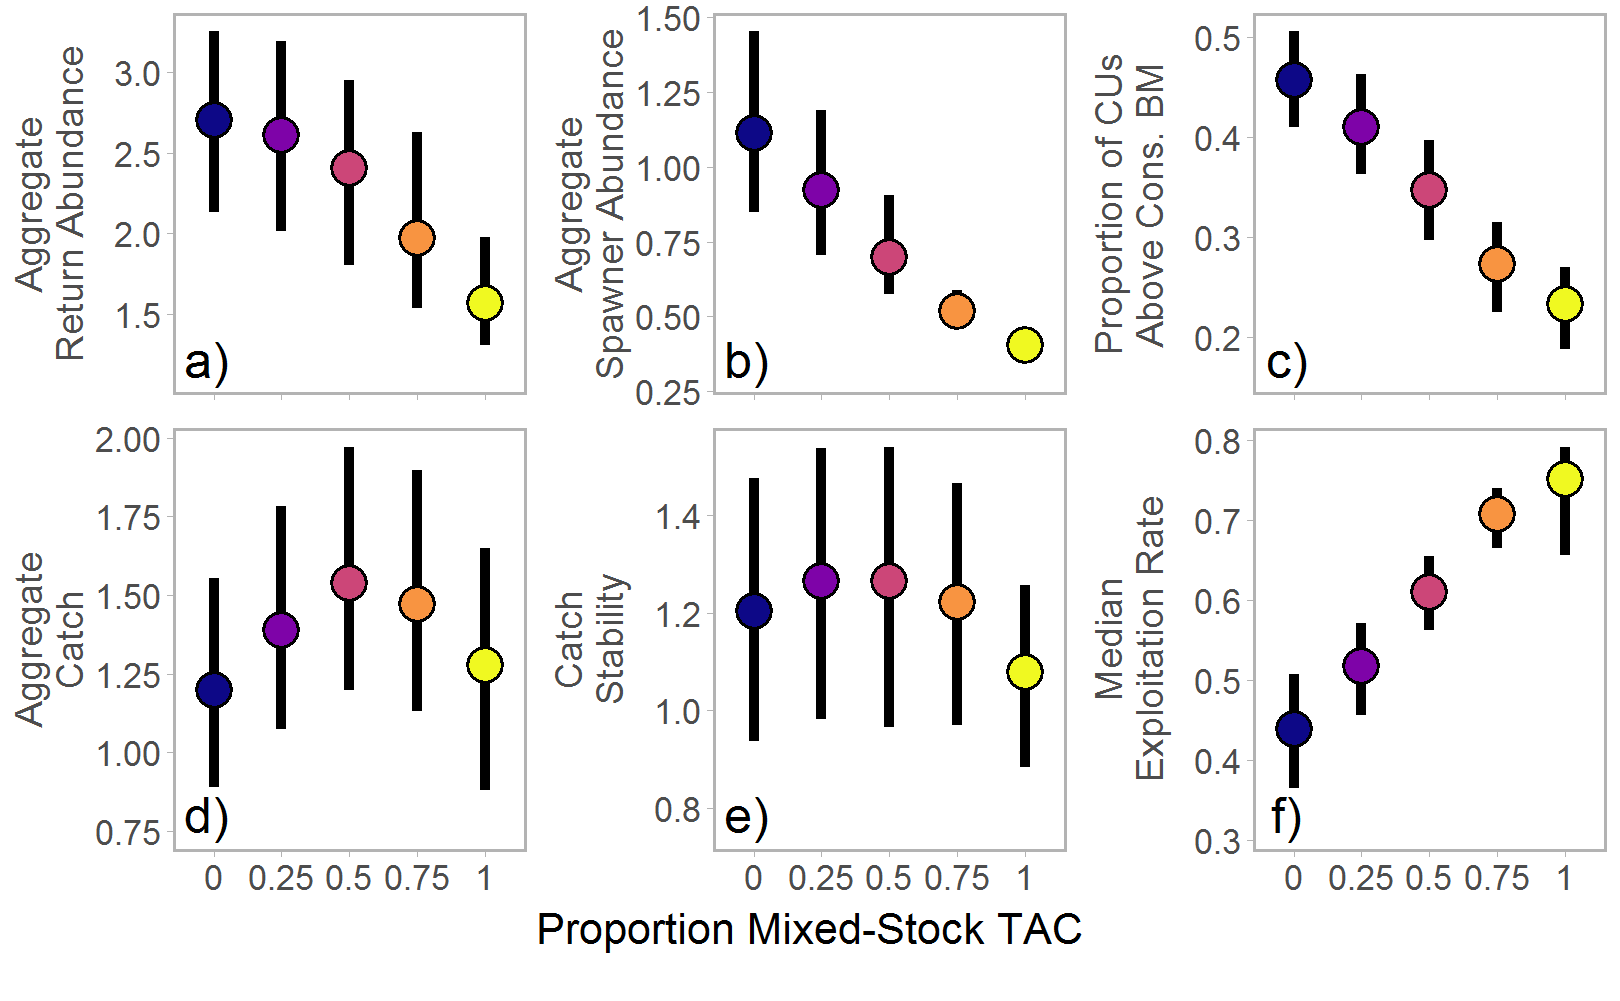
\includegraphics[width=6in]{knitr-figs-pdf/aggDot-1}}{Figure \ref{fig:aggDot}} 

}

\caption{Changes in aggregate conservation- and catch-based performance metrics across a range of fishery allocations, i.e. range of proportional allocation of mixed- to single-stock where 1 and 0 are fully mixed- and fully single-stock fisheries, respectively. Points represent medians and whiskers represent 90th percentile intervals among Monte Carlo trials.}\label{fig:aggDot}
\end{figure}
At the aggregate scale, intermediate mixed-stock allocations appeared to optimize trade-offs between conservation- and catch-based objectives. For example, splitting TAC evenly between mixed- and single-stock fisheries led to high median catches, while resulting in relatively modest declines in median return abundance (11\% decline; Fig.~\ref{fig:aggTO} left) and the mean proportion of CUs above their biological benchmark (24\% decline; Fig.~\ref{fig:aggTO} right).
\begin{figure}[htb]

{\centering \pdftooltip{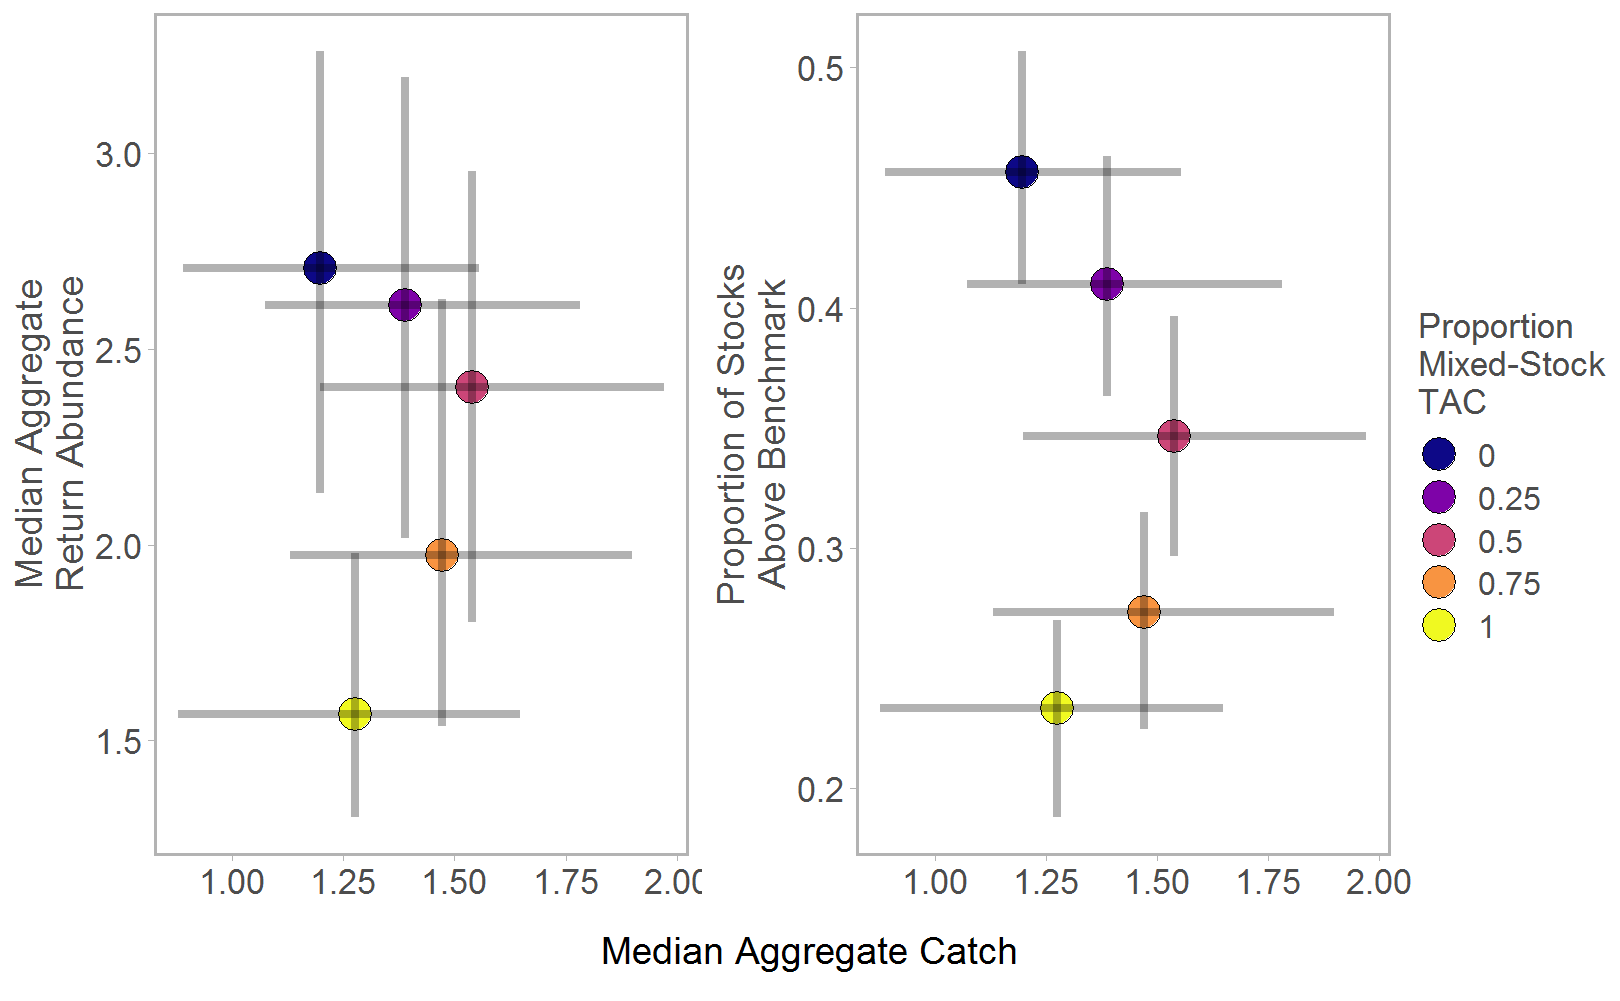
\includegraphics[width=6in]{knitr-figs-pdf/aggTO-1}}{Figure \ref{fig:aggTO}} 

}

\caption{Trade-offs between aggregate conservation- and catch-based performance metrics across a range of mixed-stock fishery allocations. Points represent medians and whiskers represent 90th percentile intervals among Monte Carlo trials.}\label{fig:aggTO}
\end{figure}
Equivalent trade-offs were more nuanced at the scale of individual CUs. For example, abundant and relatively productive stocks either were insensitive (Harrison CU, Fig.~\ref{fig:cuTO}) or responded positively (Chilko CU, Fig.~\ref{fig:cuTO}) to increases in mixed-stock fishery allocations. In both cases, single-stock fisheries are rarely closed (because the CU remained above its biological benchmark), resulting in exploitation rates that are independent of fishery allocation. In the case of the Chilko CU, the rare single-stock closures have negative impacts because they result in large spawner abundances and reduced abundance in subsequent years due to density dependent effects (i.e.~overescapement).

More commonly, however, larger mixed-stock fishery allocations resulted in declines in return abundance and ultimately catch due to recruitment overfishing (Fig.~\ref{fig:cuTO}). These effects were particularly severe in the smallest stock, Raft, which exhibited strong declines when mixed-stock fishery allocations exceeded 25\% (Fig.~\ref{fig:cuTO}). For other CUs declines in catch occurred when mixed-stock allocations exceeded 50\%.
\begin{figure}[htb]

{\centering \pdftooltip{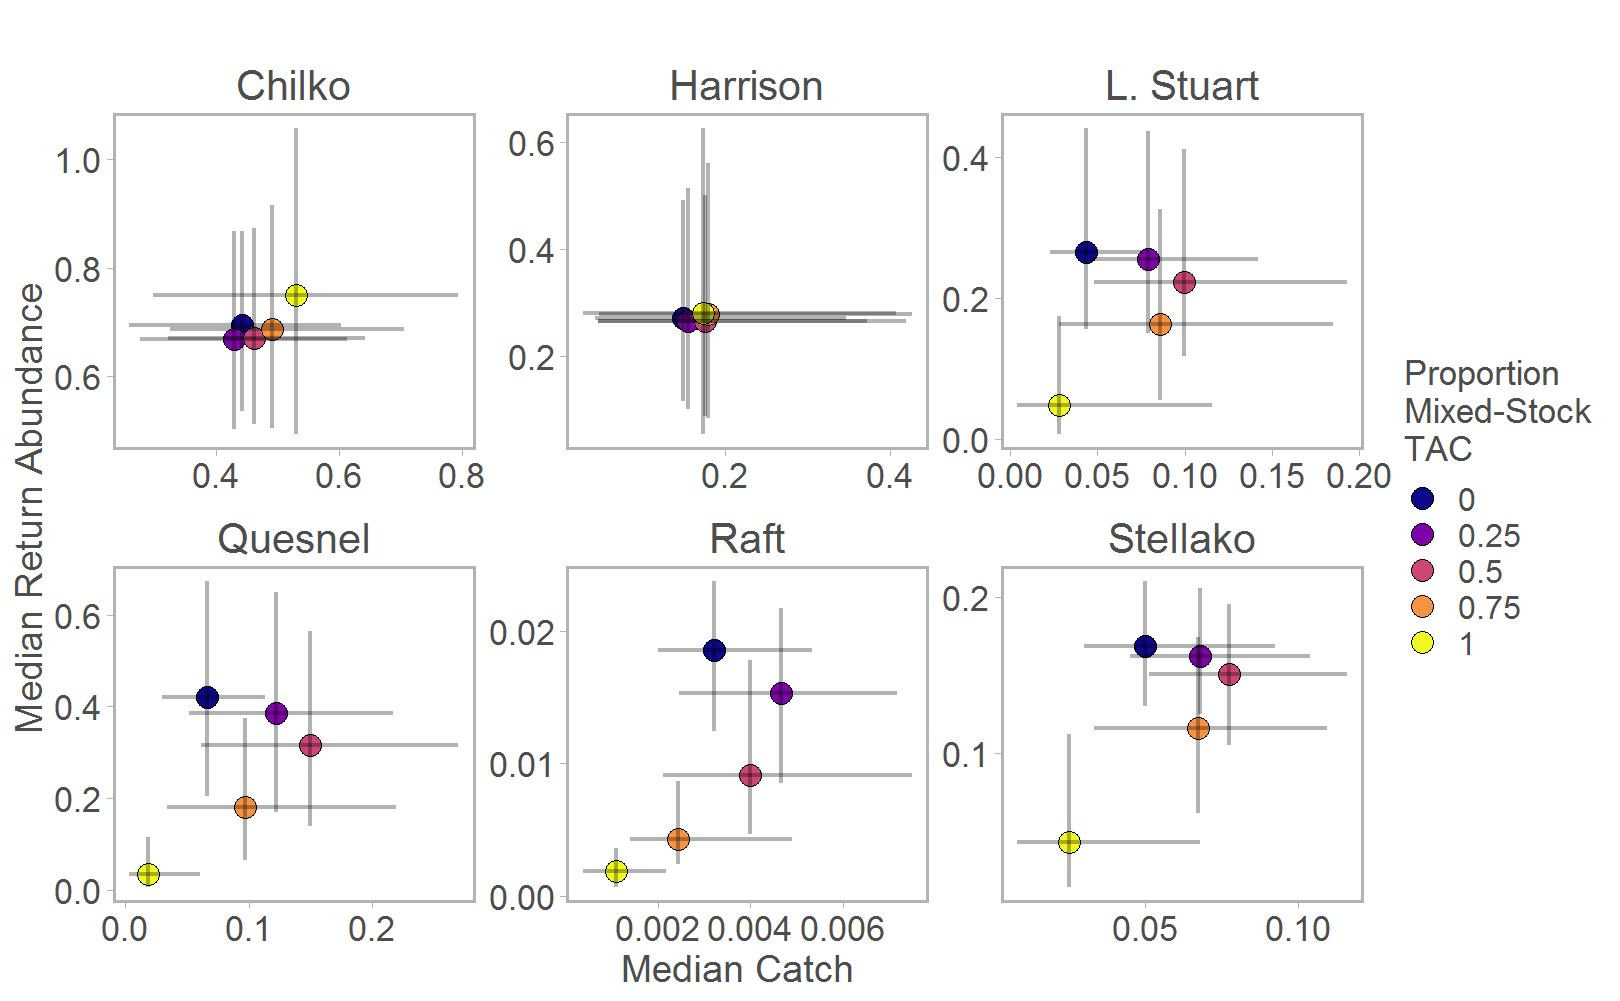
\includegraphics[width=6in]{knitr-figs-pdf/cuTO-1}}{Figure \ref{fig:cuTO}} 

}

\caption{Trade-offs between CU-specific return abundance and catch across a range of mixed-stock fishery allocations. Points represent medians and whiskers represent 90th percentile intervals among Monte Carlo trials.}\label{fig:cuTO}
\end{figure}
Changes in population productivity moderated the effect of fishery allocations on conservation- and catch-based metrics. At high levels of productivity, increasing single-stock fishery allocations resulted in relatively large increases in the proportion of stocks above \(S_{con}\); however as productivity declines the relative difference between predominantly mixed- and single-stock fishery decreases (Fig.~\ref{fig:prodTO} left). Conversely, median catch is maximized at intermediate allocations when productivity is high, but as productivity declines predominantly single-stock fisheries begin to provide greater catches (Fig.~\ref{fig:prodTO} right).
\begin{figure}[htb]

{\centering \pdftooltip{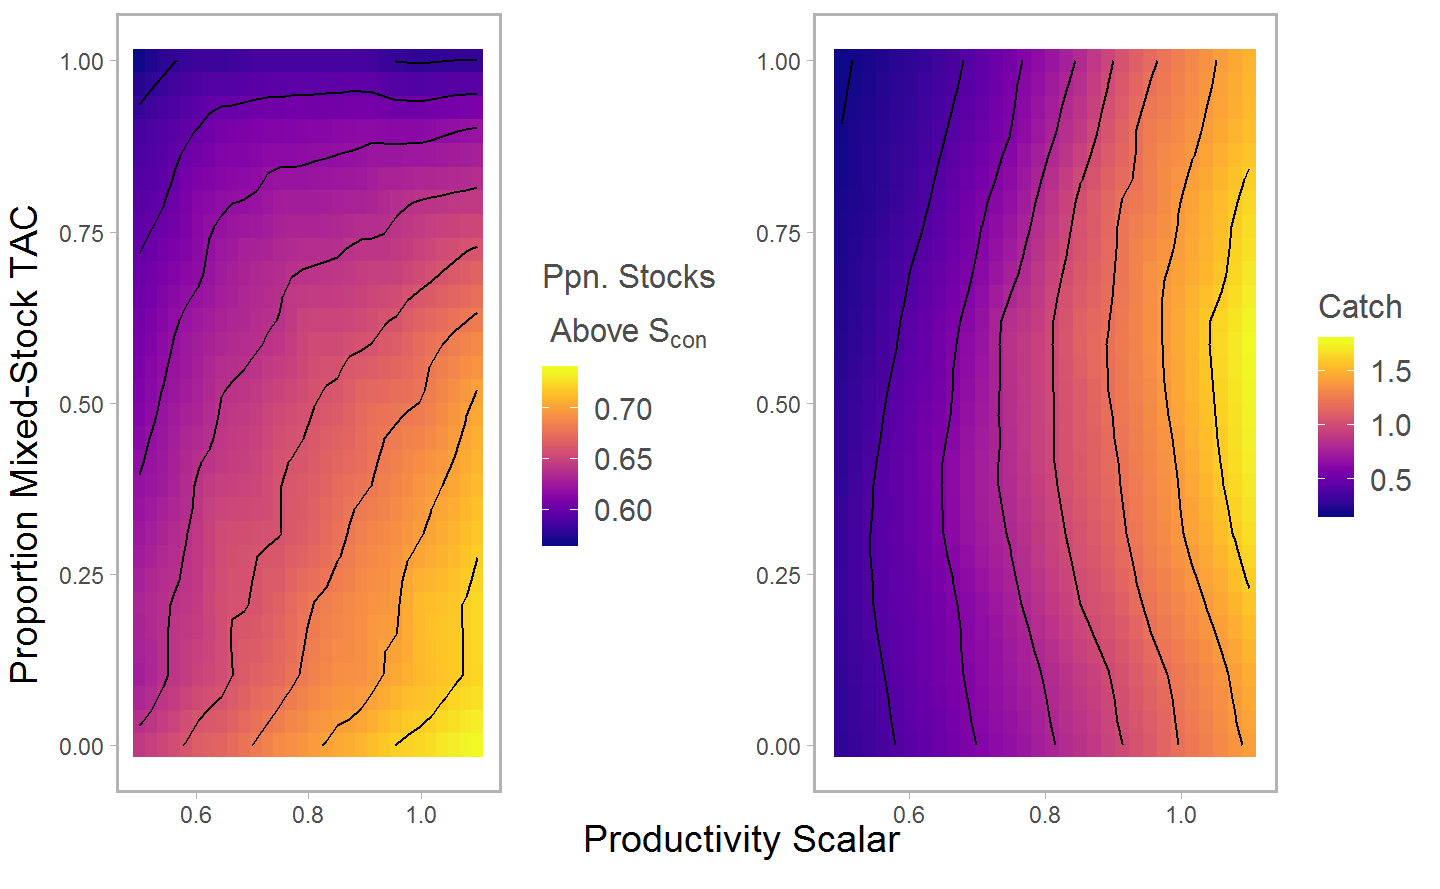
\includegraphics[width=6in]{knitr-figs-pdf/prodTO-1}}{Figure \ref{fig:prodTO}} 

}

\caption{Impacts of changes in productivity on median proportion of stocks above their biological benchmark (left) and median aggregate catch (right) across across a range of mixed-stock fishery allocations. Productivity is moderated by a scalar applied uniformly to all CU's most recent estimate of productivity.}\label{fig:prodTO}
\end{figure}
Trade-offs between mixed- and single-stock fisheries were sensitive to the structure of the harvest control rule. For example, a more precautionary mixed-stock harvest control rule, which replicated the framework currently used by Fraser River sockeye salmon managers, still resulted in larger catches in mixed-stock fisheries (relative to single-stock), but did not exhibit evidence of recruitment overfishing (i.e.~no backward bending curve) (Fig.~\ref{fig:hcrTO}). Additionally, declines in conservation-based performance metrics with predominantly mixed-stock fisheries were more modest than those observed with the reference, generic mixed-stock harvest control rule (Fig.~\ref{fig:hcrTO}).
\begin{figure}[htb]

{\centering \pdftooltip{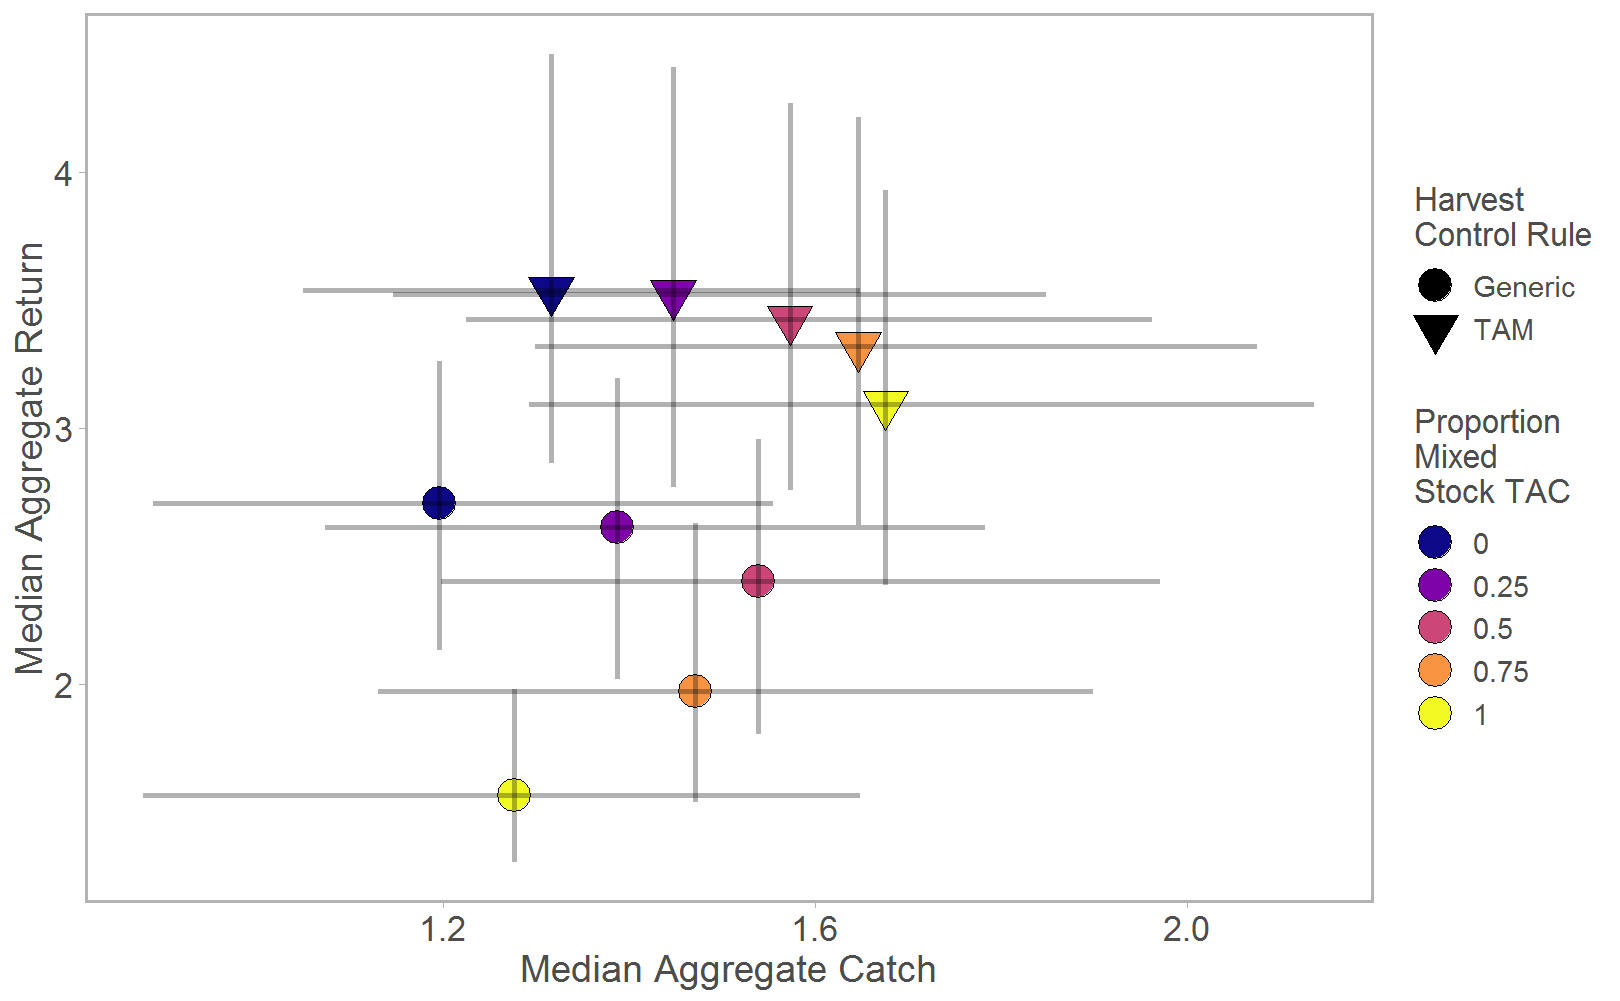
\includegraphics[width=6in]{knitr-figs-pdf/hcrTO-1}}{Figure \ref{fig:hcrTO}} 

}

\caption{Comparison of generic multi-stock harvest control rule and a more precautionary total allowable mortality (TAM) rule. Points represent medians and whiskers represent 90th percentile intervals among Monte Carlo trials.}\label{fig:hcrTO}
\end{figure}
The timing of en-route mortality also altered the trade-offs associated with fishery allocations. When en-route mortality occurred before single-stock fisheries median aggregate return abundance and the proportion of CUs above their conservation threshold in single-stock fisheries declined relative to the reference scenario (Fig.~\ref{fig:erTO}). Additionally median aggregate catch in single-stock fisheries was considerably lower (Fig.~\ref{fig:hcrTO}).
\begin{figure}[htb]

{\centering \pdftooltip{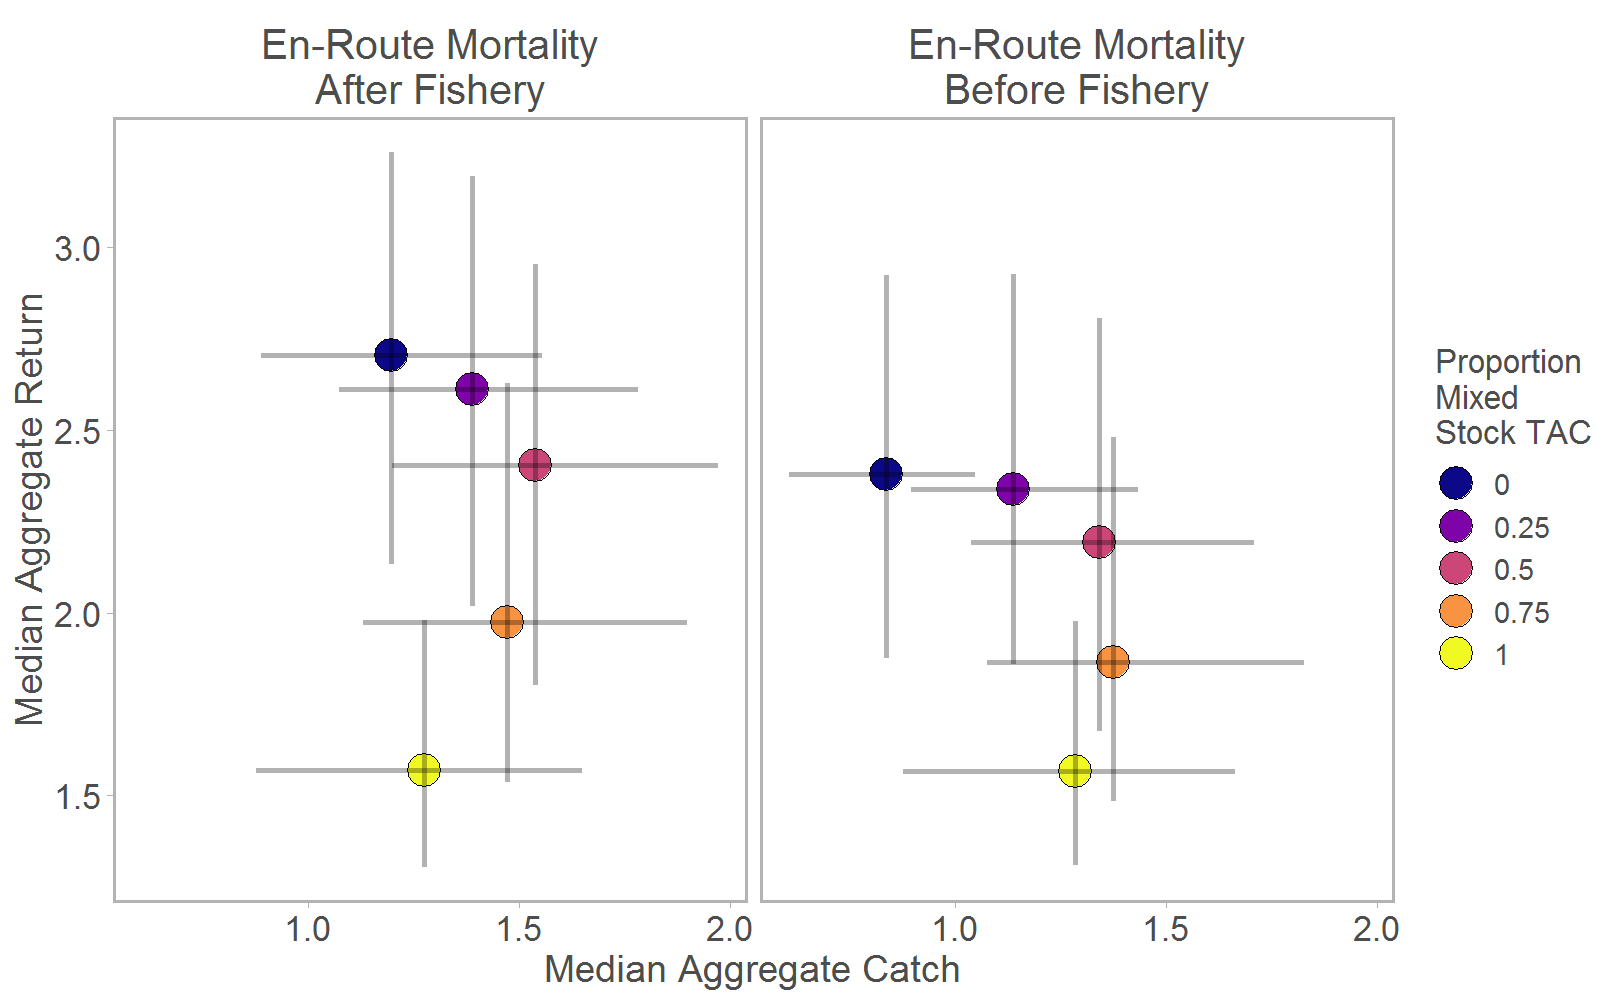
\includegraphics[width=6in]{knitr-figs-pdf/erTO-1}}{Figure \ref{fig:erTO}} 

}

\caption{The impact of en route mortality timing, relative to single-stock fisheries, on trade-offs between aggregate return abundance and catch. Points represent medians and whiskers represent 90th percentile intervals among Monte Carlo trials.}\label{fig:erTO}
\end{figure}
\section{Discussion}\label{discussion}

Shifting harvest from mixed- to single-stock fisheries may provide a means of maximizing harvest opportunities on abundant populations while minimizing risks on sympatric stocks of concern. While increasing stock selectivity has intuitive conservation benefits (Walters et al. \protect\hyperlink{ref-Walters2008}{2008}) (Atlas?), to our knowledge, the impact of such a transition on Pacific salmon fisheries has not been previously quantified. Here we used a stochastic, closed-loop simulation model to explore the trade-offs associated with catch- and conservation-based management objectives as allocations to single-stock fisheries increase. We focused on generic harvest control rules that could be readily applied to a wide range of Pacific salmon fisheries. We found that increasing allocations to single-stock fisheries resulted in improved conservation performance, albeit at the cost of reduced aggregate catches. We also determined that trade-offs between these objectives will be sensitive to the ecological scale of performance metrics, the structure of each fishery's harvest control rule, and population dynamics within the stock aggregate.

At the aggregate (i.e.~multi-stock) scale, fully single-stock fisheries maximized return abundance and the proportion of stocks above conservation benchmarks. Conversely, shifting harvest allocations entirely to mixed-stock fisheries resulted in reduced conservation performance, as well as reductions in long-term catches and catch stability due to recruitment overfishing. Intermediate allocations, which split TAC between mixed- and single-stock fisheries approximately equally, typically maximized catch metrics without substantial declines in conservation performance. These results were driven by two factors. First, single-stock fisheries were more conservative than the mixed-stock, resulting in a negative relationship between single-stock allocations and exploitation rate. Second, even though the mixed-stock harvest control rule was based on precautionary principles (i.e.~harvest rates intended to result in aggregate spawner abundance at MSY), it failed to account for temporal variability and among stock variability in productivity. As a result, fully mixed-stock allocations were more likely to result in overexploitation and declines in abundance. These patterns are consistent with evidence that harvest in mixed-stock fisheries is fundamentally constrained by the dynamics of the least productive populations (Ricker \protect\hyperlink{ref-Ricker1973}{1973}).

The impacts of single-stock fisheries are not homogeneous within an aggregate, varying among populations due to differences in intrinsic productivity and carrying capacity. While the conservation performance of smaller, less productive stocks improved as single-stock fisheries allocations increased, more productive or abundant stocks exhibited mixed responses. For example, the Harrison stock's spawner abundance regularly exceeded the biological benchmark (\(S_{con}\)) necessary to allow single-stock harvest to occur. Hence realized exploitation rates, as well as catch and conservation performance, were largely independent of fishery allocation. Conversely, the Chilko stock was actually negatively impacted by increasing single-stock fishery allocations because intermittent closures resulted in years of overescapement. Although relatively rare, these events triggered density dependent declines in both return abundance and catches.

Within our model differences among stocks are driven by variation in productivity and the magnitude of density dependent effects (i.e.~capacity). In reality, apparent differences in productivity may arise due to variation among stocks in natural mortality rates or in vulnerability to a mixed-stock fishery (Walters et al. \protect\hyperlink{ref-Walters2008}{2008}). Regardless of mechanism, such patterns suggest that the structure of fishery allocations should account for stock-specific, not just aggregate, management objectives.

Improvements in conservation performance as single-stock allocations increase will be sensitive to the underlying harvest control rules within each fishery. For example, mixed-stock Fraser River sockeye salmon fisheries are currently managed with a total allowable mortality (TAM) rule - a framework that includes a range of precautionary adjustments, as well as a maximum allowable exploitation rate (60\%) that is below estimates of \(u_{msy}\) for most stocks (Pestal et al. \protect\hyperlink{ref-Pestal2011}{2011}). When we simulated an equivalent harvest control rule, mixed-stock fisheries had no evidence of recruitment overfishing and only moderately smaller return abundances than predominantly single-stock fishery scenarios. Thus there may be minimal benefits associated with developing single-stock fisheries if mixed-stock fisheries are informed by precise in-season estimates of abundance and sufficiently precautionary. Such situations, however, may be relatively uncommon since Fraser River sockeye salmon managers have considerably more resources and data to develop detailed harvest control rules than the ``average'' salmon manager.

A wide range of single-stock fishery frameworks could be implemented, including those that maximize aggregate catch through supplementary harvest of abundant stocks in terminal areas (DFO \protect\hyperlink{ref-DFO2017a}{2017}\protect\hyperlink{ref-DFO2017a}{a}) (Atlast ref). We chose to test a relatively conservative harvest control rule, which simply closed single-stock fisheries for depleted populations, because many Canadian salmon populations are relatively data limited (Price et al. \protect\hyperlink{ref-Price2008}{2008}, Holt and Folkes \protect\hyperlink{ref-Holt2015}{2015}) and because large numbers of depleted stocks suggest diversity may be at risk (COSEWIC REFS). Under the simulated HCR, the decision to open a particular population's fishery could be made pre-season based on recent abundance relative to the time series average, even if biological benchmarks based on stock-recruit parameters cannot be estimated. We believe the model represents a management framework that could increase the probability of maintaining stock diversity with relatively small additional requirements in management capacity.

The performance of single-stock fisheries will also be sensitive to ecological processes outside of fisheries managers' control. For example, when productivity declines, even less conservative harvest control rules may result in low exploitation rates as long as they are linked to abundance. In such a scenario single-stock fisheries provided minimal additional improvements in conservation performance. Therefore, a transition to single-stock fisheries may be unlikely to resolve recent declines in salmon abundance that are linked to widespread, synchronous declines in marine survival (Peterman and Dorner \protect\hyperlink{ref-Peterman2012}{2012}, Dorner et al. \protect\hyperlink{ref-Dorner2017}{2017}). In fact, greater covariance among stocks may result in modest improvements in the performance of mixed-stock harvest control rules as stock aggregates increasingly behave like single populations (Freshwater et al. n.d.). Conversely, the performance of single-stock fisheries is likely to improve if productivity patterns within a stock aggregate diverge and abundant populations can be effectively targeted.

Options to increase stock selectivity are limited when a salmon aggregate contains large numbers of populations that share similar migration phenologies (Walters et al. \protect\hyperlink{ref-Walters2008}{2008}). In such a situation developing single-stock fisheries likely requires moving harvest to terminal areas, however these fisheries may require additional management considerations. First adult fish will recruit into the fishery only after completing their freshwater migrations. Since en route mortality rates can exceed 90\% in certain years (Cooke et al. \protect\hyperlink{ref-Cooke2004}{2004}), terminal single-stock fisheries will have access to less harvestable biomass than downstream marine fisheries, resulting in reduced catches. Furthermore, management uncertainty in terminal fisheries, which may increase if precise estimates of spawner abundance are not available for all stocks, could have particularly severe impacts if stocks are at low abundance due to en route mortality.

The decision to change allocations between mixed- and single-stock fisheries will ultimately need to incorporate a broad range of socio-economic factors. For example, the landed value per weight of catches in terminal areas will almost certainly be lower than marine caught fish because individuals expend large portions of their energy reserves while migrating. Perhaps more importantly, increasing single-stock harvest would result in dramatic changes in access among user groups. Ideally a full management strategy evaluation, incorporating all major user groups, could be used to specify socio-economic objectives, then quantify trade-offs prior to changes in allocation. Nevertheless, these simulations demonstrate that the probability of meeting conservation objectives can be improved by increasing stock selectivity using relatively simple harvest control rules.

\Appendices

\clearpage

\refstepcounter{chapter}

\starredchapter{APPENDIX~\thechapter. Appendix S1}\label{app:appendixS1}

\appsection{Larkin model}\label{larkin-model}

Cyclic salmon stocks are typically modeled using an adaptation of the Ricker model, the Larkin model, featuring delayed density-dependence parameters (Larkin \protect\hyperlink{ref-Larkin1971}{1971})

Equation S1 \[log(\frac{R_{i,y}}{S_{i,y}}) = \alpha_i - \beta_iS_{i,y} - \beta_{1,i}S_{i,y-1} - \beta_{2,i}S_{i,y-2} - \beta_{3,i}S_{i,y-3} + w_{i,y}\]

where \(i\) represents a stock, \(y\) is a given brood year, \(R\) the number of recruits, and \(S\) the number of spawners. The parameter \(\alpha\) represents the number of recruits produced per spawner at low abundance, while \(\beta_{x}\) is the density-dependent parameter at time lag \(x\). Stochastic recruitment deviations, \(w_{i,y}\), are normally distributed with mean zero and variance \(\sigma^2\).

\appsection{Recursive Bayes stock-recruit model}\label{recursive-bayes-stock-recruit-model}

\appsection{Harvest control rules}\label{harvest-control-rules}

As described in the main text, the simulation model generated target harvest rates (for both fisheries combined) using a generic, abundance-based harvest control rule (HCR) proposed under Fisheries and Oceans Canada's Precautionary Approach Framework (DFO \protect\hyperlink{ref-DFO2017b}{2017}\protect\hyperlink{ref-DFO2017b}{b}). Specifically a minimal exploitation rate (10\%) approximating incidental harvest was applied when MU-level abundance was less than 40\% of the spawner abundance that would lead to maximumum sustainable yield (\(0.4{S}_{MSY}\)). When abundance was greater than 80\% of that spawner abundance (\(0.8{S}_{MSY}\)), the exploitation rate at maximum sustainable yield (approximated by \({u}_{MSY}\); Fig.~\ref{fig:genHCR}) was applied. When return abundance was between these two reference points, the target exploitation rate was a linear function of abundance (Fig.~\ref{fig:genHCR}).
\begin{figure}[htb]

{\centering \pdftooltip{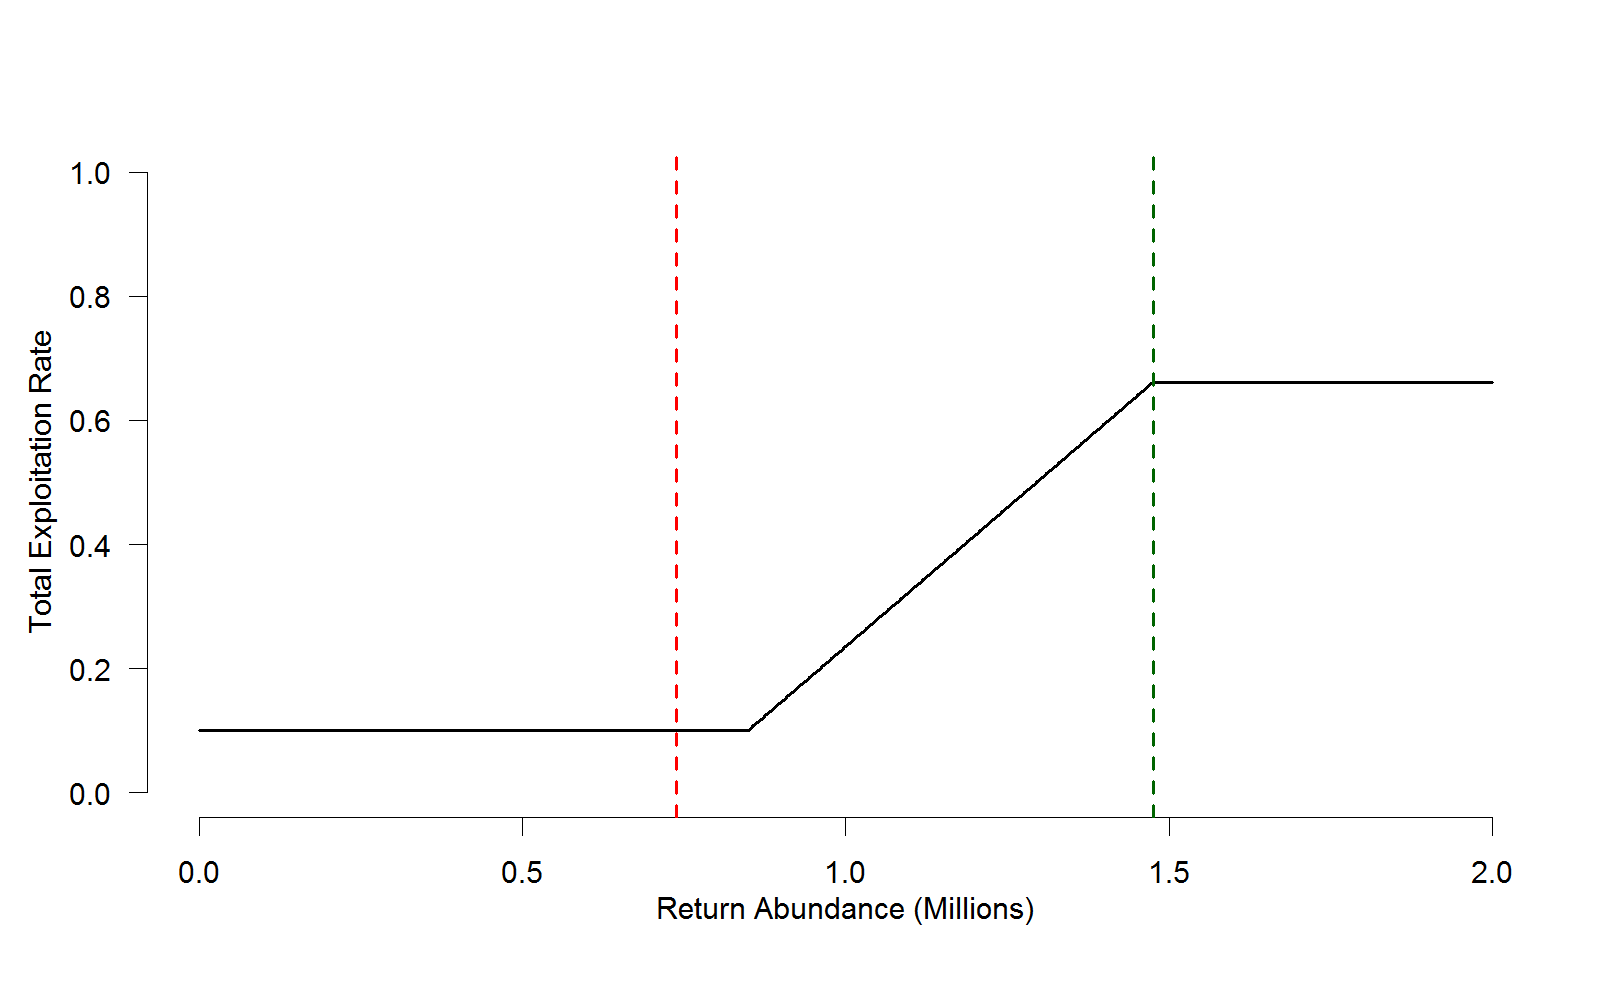
\includegraphics[width=6in]{knitr-figs-pdf/genHCR-1}}{Figure \ref{fig:genHCR}} 

}

\caption{Generic, abundance-based harvest control rule used to calculate target exploitation rates. Dashed vertical lines represent lower (red) and upper (green) fishery reference points equivalent to $0.4{S}_{MSY}$ and $0.8{S}_{MSY}$, respectively. The maximum exploitation rate is equal to ${u}_{MSY}$.}\label{fig:genHCR}
\end{figure}
We also evaluated the impact of an alternative HCR, a total allowable mortality (TAM) rule, intended to approximate the management framework currently used for Fraser River sockeye salmon. As with the reference HCR, the TAM rule specifies annual target harvest rates based return abundance relative to two fishery reference points. Unlike the generic HCR, however, the TAM rule reference points differ vary among cycle lines, are derived using expert knowledge, and the maximum target harvest rates are lower (Table~\ref{tab:frpTable}).
\begin{longtable}[]{@{}lrrrr@{}}
\caption{\label{tab:frpTable}Fishery reference points (FRP; in millions of fish) and maximum exploitation rates (ER) for the generic harvest control rule utilized in the main text and the total allowable mortality rule.}\tabularnewline
\toprule
Harvest Control Rule & Cycle & Low FRP & High FRP & Maximum ER\tabularnewline
\midrule
\endfirsthead
\toprule
Harvest Control Rule & Cycle & Low FRP & High FRP & Maximum ER\tabularnewline
\midrule
\endhead
Generic & NA & 0.74 & 1.48 & 0.66\tabularnewline
TAM & 1 & 0.89 & 1.24 & 0.60\tabularnewline
& 2 & 1.02 & 1.43 & 0.60\tabularnewline
& 3 & 0.76 & 1.06 & 0.60\tabularnewline
& 4 & 0.64 & 0.90 & 0.60\tabularnewline
\bottomrule
\end{longtable}
The TAM rule also differs from the generic HCR due to two additional adjustments. First, harvest rates are typically lowered due to anticipated en-route mortality. We simulated this process by applying an en-route mortality adjustment, \emph{pMA}, that acts as a scalar on escapement goals (i.e.~a \emph{pMA} equal to 0 is no adjustment, equal to 1 is a 100\% increase in the escapement goal). We parameterized this model component by setting the \emph{pMA} equal to the median \emph{pMA} observed for the Summer Run MU since 2000. Harvest rates are also adjusted annually to reduce incidental harvest of co-migrating MUs that are at low abundance. However, we excluded this adjustment because we only modeled one MU (Summer Run stocks).

\clearpage

\refstepcounter{chapter}

\starredchapter{APPENDIX~\thechapter. Appendix S2}\label{app:appendixS2}

\appsection{Multistock fishery harvest control rule}\label{multistock-fishery-harvest-control-rule}

\emph{Move from main text based on co-author comments.}

\appsection{En-route mortality}\label{en-route-mortality}

\emph{Move from main text based on co-author comments.}

\appsection{Stochastic parameter sensitivity analyses}\label{stochastic-parameter-sensitivity-analyses}

We used local sensitivity analyses to evaluate how our conclusions may be impacted by the magnitude of interannual variation in stochastic parameters and temporal autocorrelation. For each parameter we selected upper and lower values (bounding plausible ranges; Table S1), held the remaining parameters constant, and compared distributions of performance metrics generated from 1500 Monte Carlo trials. We present results from a management procedure specifying equal allocations between mixed- and single-stock fisheries for all sensitivity scenarios. Additional analyses indicated that increasing the mixed-stock allocation increased the effect of mixed-stock fishery outcome uncertainty, while reducing the effect of single-stock outcome uncertainty. The opposite pattern occurred when single-stock fishery allocations were increased. Since the overall patterns remained similar these results are not shown.

To evaluate interannual variability in age-at-maturity and en-route mortality we applied scalars to \(\Omega\) and \(\sigma_{mort}\) cosnsitent with stock-specific differences (i.e.~were within on standard deviation of observed values; Table S2). To evaluate the sensitivity of fishery-specific outcome uncertainty we set the lower value for \(\sigma_{out}\) at zero (i.e.~no deviations between target and realized catch) and the maximum value at 0.15, an arbitrary value resulting in \textasciitilde{}20\% of harvest rate deviations exceeding the maxmimum deviation observed among all Fraser River sockeye salmon management units between 2006 and 2017. Conversely, the reference \(\sigma_{out}\) (0.07) results in \textasciitilde{}0.2\% of deviations exceeding the maximum observed. We applied the same minimum and maximum values to both single- and mixed-stock fisheries, but did so independently. Finally, we set the minimum temporal autocorrelation \(\tau\) value at zero and the maximum at the largest estimated value from a study of Alaskan sockeye salmon (Peterman et al. \protect\hyperlink{ref-Peterman2003}{2003}).

The effects of greater variability differed among stochastic parameters and performance metrics. Greater outcome uncertainty within mixed-stock fisheries had the most consistent negative impact, with larger deviations between realized and target catch resulting in declines in all performance metrics (Fig.~\ref{fig:sensPlot}). Such patterns are consistent with evidence that outcome uncertainty can limit conservation and harvest objectives (Holt and Peterman \protect\hyperlink{ref-Holt2006}{2006}). Conversely, greater single-stock fishery outcome uncertainty had a relative modest impact, particularly on spawner abundance, because the single-stock fishery had zero harvest when abundance was low (Fig.~\ref{fig:sensPlot}).

Greater temporal autocorrelation in recruitment deviations led to declines in recruitment, escapement, the proportion of stocks above their biological benchmark, and catch (Fig.~\ref{fig:sensPlot}). Such patterns are likely due to temporal autocorrelation weakening compensatory biological and management processes. Changes in interannual variability in maturation age and en route mortality rates had relatively minor effects on all performance metrics. Regardless of the performance metric, however, 90\% quantile intervals for each sensitivity scenario overlapped the reference opearting model (Fig.~\ref{fig:sensPlot}). Since this pattern was stable when allocations were fully single- or fully mixed-stock, our conclusions are unlikely to be biased by the magnitude of stochastic parameters.

\textbackslash{}begin\{figure\}{[}htb{]}

\{\centering \pdftooltip{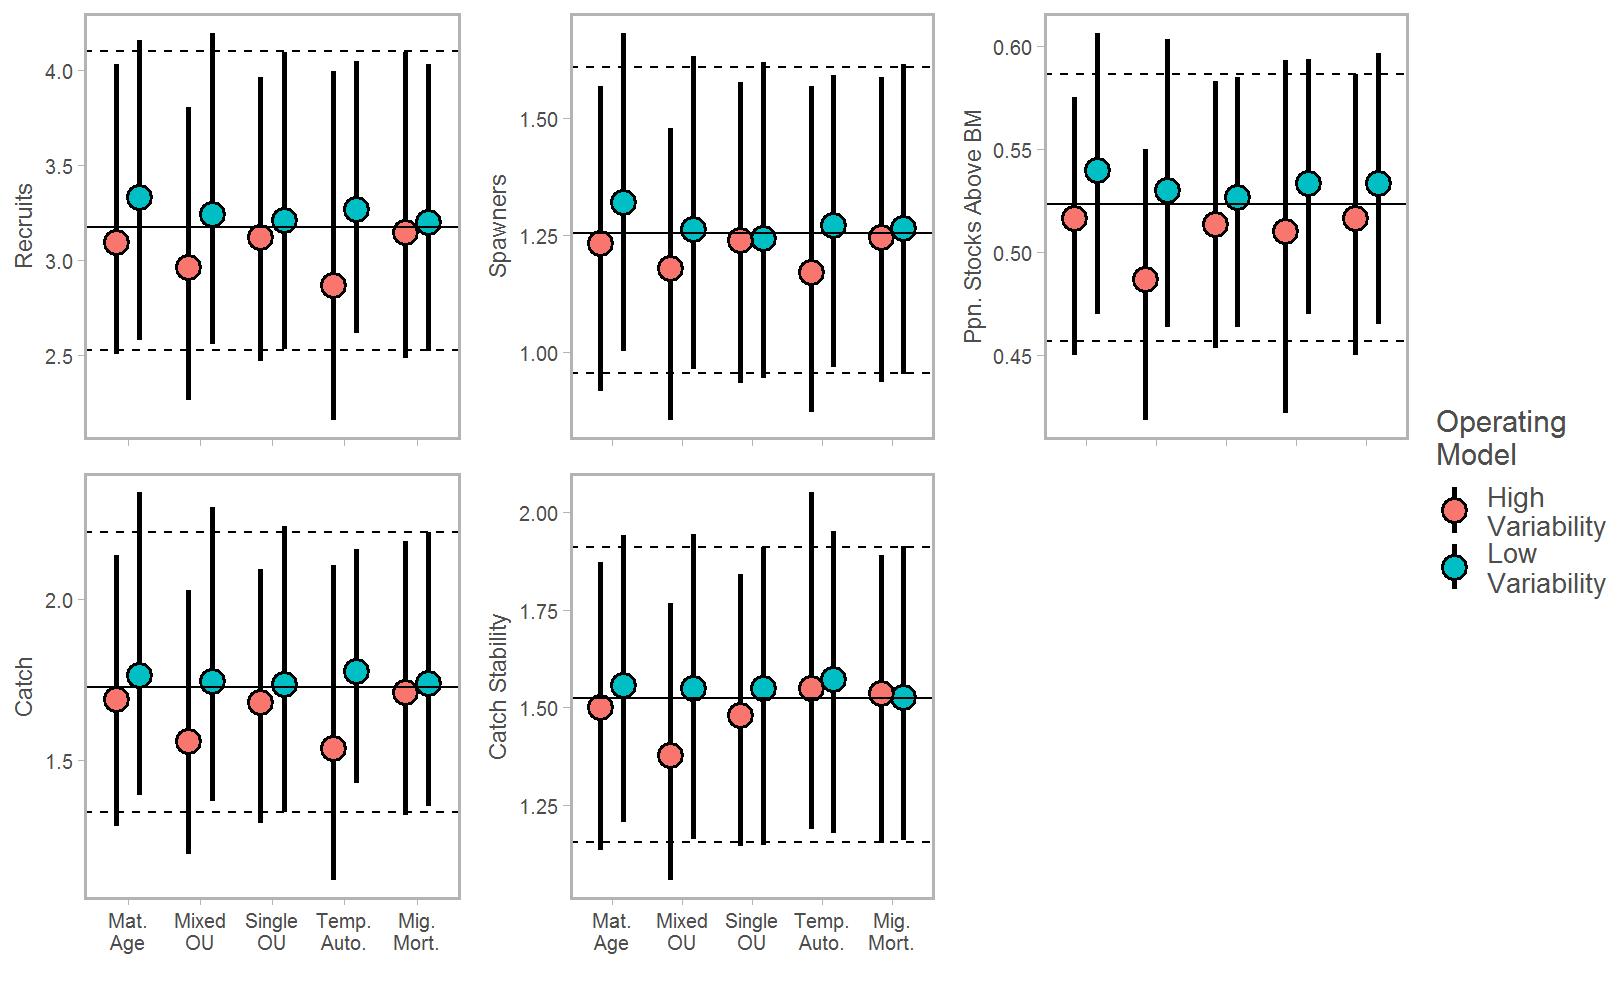
\includegraphics[width=6in]{knitr-figs-pdf/sensPlot-1}}{Figure \ref{fig:textbackslash{}caption{[}Sensitivity of conservation- and catch-based performance metrics to stochastic parameters and temporal autocorrelation{]}{Sensitivity of conservation- and catch-based performance metrics to stochastic parameters and temporal autocorrelation. All scenarios assume a 50% of the total allowable catch was allocated to each fishery. Horizontal lines represent the median (solid) estimate and 90th percentile intervals (dashed) from the reference operating model. Points represent medians and whiskers represent 90th percentile intervals among Monte Carlo trials.}label{fig:sensPlot} textbackslash{}end{figure}}}

\}

\textbackslash{}caption{[}Sensitivity of conservation- and catch-based performance metrics to stochastic parameters and temporal autocorrelation{]}\{Sensitivity of conservation- and catch-based performance metrics to stochastic parameters and temporal autocorrelation. All scenarios assume a 50\% of the total allowable catch was allocated to each fishery. Horizontal lines represent the median (solid) estimate and 90th percentile intervals (dashed) from the reference operating model. Points represent medians and whiskers represent 90th percentile intervals among Monte Carlo trials.\}\label{fig:sensPlot} \textbackslash{}end\{figure\}

\clearpage

\section*{REFERENCES}\label{references}
\phantomsection
\addcontentsline{toc}{section}{REFERENCES}
% This manually sets the header for this unnumbered chapter.
\noindent
\vspace{-2em}
\setlength{\parindent}{-0.2in}
\setlength{\leftskip}{0.2in}
\setlength{\parskip}{8pt}

\hypertarget{refs}{}
\hypertarget{ref-Anderson2015}{}
Anderson, S. C., W. M. Jonathan, M. M. Michelle, K. D. Nicholas, and B. C. Andrew. 2015. Portfolio conservation of metapopulations under climate change. Ecological Applications 25:559--572.

\hypertarget{ref-Burgner1991}{}
Burgner, R. L. 1991. Life history of Sockeye Salmon (Oncorhynchus nerka). \emph{in} C. Groot and L. Margolis, editors. Pacific salmon life histories. University of British Columbia Press, Vancouver, B.C.

\hypertarget{ref-Cohen2012}{}
Cohen, B. I. 2012. The Uncertain Future of Fraser River Sockeye - Part 1. Cohen Commission 1:692.

\hypertarget{ref-Cooke2004}{}
Cooke, S. J., S. G. Hinch, A. P. Farrell, M. F. Lapointe, S. R. M. Jones, J. S. Macdonald, D. A. Patterson, M. C. Healey, and G. van der Kraak. 2004. Abnormal migration timing and high en route mortality of sockeye salmon in the Fraser River, British Columbia. Fisheries Research 29:22--33.

\hypertarget{ref-COSEWIC2017}{}
COSEWIC. 2017. COSEWIC assessment and status report on the Sockeye Salmon Oncorhynchus nerka, 24 Designatable Units in the Fraser River Drainage Basin, in Canada. Committe on the Status of Endangered Wildlife In Canada:179 p.

\hypertarget{ref-cunninghamPress}{}
Cunningham, C. J., C. M. Anderson, J. Y.-l. Wang, M. R. Link, and R. Hilborn. (n.d.). A management strategy evaluation of the commercial sockeye salmon fishery in Bristol Bay, Alaska. Canadian Journal of Fisheries \& Aquatic Sciences.

\hypertarget{ref-Cunningham2017}{}
Cunningham, C. J., T. A. Branch, T. H. Dann, M. Smith, J. E. Seeb, L. W. Seeb, and R. Hilborn. 2017. A general model for salmon run reconstruction that accounts for interception and differences in availability to harvest. Canadian Journal of Fisheries and Aquatic Sciences 13:1--13.

\hypertarget{ref-DFO2005}{}
DFO. 2005. Canada's Policy for Conservation of Wild Pacific Salmon. Fisheries; Oceans Canada.

\hypertarget{ref-DFO2017a}{}
DFO. 2017a. Integrated Fisheries Management Plan: June 1, 2017 - May 31, 2017. Fisheries; Oceans Canada.

\hypertarget{ref-DFO2017b}{}
DFO. 2017b. Guidance for the development of rebuilding plans under the Precautionary Approach Framework: Growing stocks out of the critical zone.

\hypertarget{ref-Dorner2017}{}
Dorner, B., M. J. Catalano, and R. M. Peterman. 2017. Spatial and temporal patterns of covariation in productivity of Chinook salmon populations of the Northeastern Pacific. Canadian Journal of Fisheries and Aquatic Sciences 1095:cjfas--2017--0197.

\hypertarget{ref-FreshwaterSub}{}
Freshwater, C., S. A. Anderson, K. R. Holt, A.-M. Huang, and C. A. Holt. (n.d.). Weakened portfolio effects constrain management effectiveness for population aggregates. Ecological Applications.

\hypertarget{ref-Freshwater2018}{}
Freshwater, C., B. J. Burke, M. D. Scheuerell, S. C. H. Grant, M. Trudel, and F. Juanes. 2018. Coherent population dynamics associated with sockeye salmon juvenile life history strategies. Canadian Journal of Fisheries and Aquatic Science 75:1346--1356.

\hypertarget{ref-Grant2011}{}
Grant, S. C. H., B. L. MacDonald, T. E. Cone, C. A. Holt, A. Cass, E. J. Porszt, J. M. B. Hume, and L. B. Pon. 2011. Evaluation of uncertainty in Fraser Sockeye (Oncorhynchus nerka) wild salmon policy status using abundance and trends in abundance metrics. Candian Science Advisory Secretariat Research Document 2011/087.

\hypertarget{ref-Hilborn1985}{}
Hilborn, R. 1985. Apparent stock recruitment relationships in mixed stock fisheries. Canadian Journal of Fisheries \& Aquatic Sciences:718--723.

\hypertarget{ref-Hilborn2003}{}
Hilborn, R., T. P. Quinn, D. E. Schindler, and D. E. Rogers. 2003. Biocomplexity and fisheries sustainability. Proceedings of the National Academy of Sciences 100:6564--6568.

\hypertarget{ref-Holt2010}{}
Holt, C. A. 2010. Will depleted populations of Pacific salmon recover under persistent reductions in survival and catastrophic mortality events? ICES Journal of Marine Science 67:2018--2026.

\hypertarget{ref-Holt2011}{}
Holt, C. A., and M. J. Bradford. 2011. Evaluating benchmarks of population status for Pacific salmon. North American Journal of Fisheries Management 31:363--378.

\hypertarget{ref-Holt2015}{}
Holt, C. A., and M. J. P. Folkes. 2015. Cautions on using percentile-based benchmarks of status for data-limited populations of Pacific salmon under persistent trends in productivity and uncertain outcomes from harvest management. Fisheries Research 171:188--200.

\hypertarget{ref-Holt2006}{}
Holt, C. A., and R. M. Peterman. 2006. Missing the target: uncertainties in achieving management goals in fisheries on Fraser River, British Columbia, sockeye salmon (Oncorhynchus nerka). Canadian Journal of Fisheries and Aquatic Sciences 63:2722--2733.

\hypertarget{ref-Holt2008}{}
Holt, C. A., and R. M. Peterman. 2008. Uncertainties in population dynamics and outcomes of regulations in sockeye salmon (Oncorhynchus nerka) fisheries: implications for management. Canadian Journal of Fisheries and Aquatic Sciences 65:1459--1474.

\hypertarget{ref-Holt2009}{}
Holt, C. A., A. Cass, B. Holtby, and B. Riddell. 2009. Indicators of status and benchmarks for Conservation Units in Canada's Wild Salmon Policy. CSAS Research Document 2009/058.

\hypertarget{ref-KHolt2011}{}
Holt, K. R., R. M. Peterman, and S. P. Cox. 2011. Trade-offs between monitoring objectives and monitoring effort when classifying regional conservation status of Pacific salmon (Oncorhynchus spp.) populations. Canadian Journal of Fisheries and Aquatic Sciences 68:880--897.

\hypertarget{ref-Larkin1971}{}
Larkin, P. A. 1971. Simulation studies of Adams River sockeye salmon (Oncorhynchus nerka). Journal Fisheries Research Board of Canada 28:1493--1502.

\hypertarget{ref-Link2018}{}
Link, J. S. 2018. System-level optimal yield: increased value, less risk, improved stability, and better fisheries. Canadian Journal of Fisheries and Aquatic Sciences 16:1--16.

\hypertarget{ref-Martins2012}{}
Martins, E. G., S. G. Hinch, S. J. Cooke, and D. A. Patterson. 2012. Climate effects on growth, phenology, and survival of sockeye salmon (Oncorhynchus nerka): a synthesis of the current state of knowledge and future research directions. Reviews in Fish Biology and Fisheries 22:887--914.

\hypertarget{ref-Pestal2011}{}
Pestal, G., A.-M. Huang, and A. Cass. 2011. Updated methods for assessing harvest rules for Fraser River sockeye salmon (Oncorhynchus nerka). Can. Sci. Advis. Sec. Res. Doc. 2011/133:viii + 175.

\hypertarget{ref-Peterman2012}{}
Peterman, R. M., and B. Dorner. 2012. A widespread decrease in productivity of sockeye salmon (Oncorhynchus nerka) populations in western North America. Canadian Journal of Fisheries and Aquatic Sciences 69:1255--1260.

\hypertarget{ref-Peterman2003}{}
Peterman, R. M., B. J. Pyper, and B. W. MacGregor. 2003. Use of the Kalman filter to reconstruct historical trends in productivity of Bristol Bay sockeye salmon (Oncorhynchus nerka). Canadian Journal of Fisheries and Aquatic Sciences 60:809--824.

\hypertarget{ref-Price2008}{}
Price, M. H. H., C. T. Darimont, N. F. Temple, and S. M. MacDuffee. 2008. Ghost runs: management and status assessment of Pacific salmon (Oncorhynchus spp.) returning to British Columbia's central and north coasts. Canadian Journal of Fisheries and Aquatic Sciences 65:2712--2718.

\hypertarget{ref-Punt2016}{}
Punt, A. E., D. S. Butterworth, C. L. de Moor, J. A. A. De Oliveira, and M. Haddon. 2016. Management strategy evaluation: best practices. Fish and Fisheries 17:303--334.

\hypertarget{ref-Reiss2009}{}
Reiss, H., G. Hoarau, M. Dickey-Collas, and W. J. Wolff. 2009. Genetic population structure of marine fish: mismatch between biological and fisheries management units. Fish and Fisheries 10:361--395.

\hypertarget{ref-Ricker1958}{}
Ricker, W. E. 1958. Maximum sustained yields from fluctuating environments and mixed stocks. Fisheries Research Board of Canada 15:991--1006.

\hypertarget{ref-Ricker1973}{}
Ricker, W. E. 1973. Two mechanisms that make it impossible to maintain peak-period yields from stocks of Pacific salmon and other fishes. Journal Fisheries Research Board of Canada 30:1275--1286.

\hypertarget{ref-Ricker1975}{}
Ricker, W. E. 1975. Computation and interpretation of biological statistics of fish populations. Fisheries Research Board of Canada Bulletin 191.

\hypertarget{ref-Scheuerell2016}{}
Scheuerell, M. D. 2016. An explicit solution for calculating optimum spawning stock size from Ricker's stock recruitment model. PeerJ 4:e1623.

\hypertarget{ref-Schindler2010}{}
Schindler, D. E., R. Hilborn, B. Chasco, C. P. Boatright, T. P. Quinn, L. A. Rogers, and M. S. Webster. 2010. Population diversity and the portfolio effect in an exploited species. Nature 465:609--612.

\hypertarget{ref-Schnute1995}{}
Schnute, J. T., and L. J. Richards. 1995. The influence of error on population estimates from catch-age models. Canadian Journal of Fisheries and Aquatic Sciences 52:2063--2077.

\hypertarget{ref-Stephenson2002a}{}
Stephenson, R. L. 2002. Stock structure and management structure: an ongoing challenge for ICES. ICES Marine Science Symposia 215:305--314.

\hypertarget{ref-Szuwalski2016}{}
Szuwalski, C. S., and A. B. Hollowed. 2016. Climate change and non-stationary population processes in fisheries management. ICES Journal of Marine Science 73:1297--1305.

\hypertarget{ref-Walters2019}{}
Walters, C., K. English, J. Korman, and R. Hilborn. 2019. The managed decline of British Columbia's commercial salmon fishery. Marine Policy 101:25--32.

\hypertarget{ref-Walters2008}{}
Walters, C., J. Lichatowich, R. Peterman, and J. Reynolds. 2008. Report of the Skeena Independent Science Review Panel:144.

\setlength{\parindent}{0in} \setlength{\leftskip}{0in} \setlength{\parskip}{4pt}

\markboth{References}{References}

\noindent
\vspace{-2em} \setlength{\parindent}{-0.2in} \setlength{\leftskip}{0.2in} \setlength{\parskip}{8pt}

\end{document}
